%%%%%%%%%%%%%%%%%%%%%%%%%%%%%%%%%%%%%%%%%%%%%%%%%%%%%%%%%%%%%%%%%%%%%%
% njuthesis 示例模板 v1.4.2 2024-11-08
% https://github.com/nju-lug/NJUThesis
%
% 贡献者
% Yu XIONG @atxy-blip   Yichen ZHAO @FengChendian
% Song GAO @myandeg     Chang MA @glatavento
% Yilun SUN @HermitSun  Yinfeng LIN @linyinfeng
% Yukai Chou @Muzimuzhi
%
% 许可证
% LaTeX Project Public License（版本 1.3c 或更高）
%%%%%%%%%%%%%%%%%%%%%%%%%%%%%%%%%%%%%%%%%%%%%%%%%%%%%%%%%%%%%%%%%%%%%%

%---------------------------------------------------------------------
% 一些提升使用体验的小技巧：
%   1. 请务必使用 UTF-8 编码编写和保存本文档
%   2. 请务必使用 XeLaTeX 或 LuaLaTeX 引擎进行编译
%   3. 不保证接口稳定，写作前一定要留意版本号
%   4. 以百分号(%)开头的内容为注释，可以随意删除
%---------------------------------------------------------------------

%---------------------------------------------------------------------
% 请先阅读使用手册：
% http://mirrors.ctan.org/macros/unicodetex/latex/njuthesis/njuthesis.pdf
%---------------------------------------------------------------------

\documentclass[
    % 模板选项(注意右端逗号)：
    %
    % type = bachelor|master|doctor|postdoc, % 文档类型，默认为本科生
    % degree = academic|professional,        % 学位类型，默认为学术型
    %
    % nl-cover,   % 是否需要国家图书馆封面，默认关闭
    % decl-page,  % 是否需要诚信承诺书或原创性声明，默认关闭
    %
    %   页面模式，详见手册说明
    % draft,                  % 开启草稿模式
    % anonymous,              % 开启盲审模式
    % minimal,                % 开启最小化模式
    %
    %   单双面模式，默认为适合印刷的双面模式
    oneside,                % 单面模式，无空白页
    % twoside,                % 双面模式，每一章从奇数页开始
    %
    %   字体设置，不填写则自动调用系统预装字体，详见手册
    fontset = win, % |mac|macoffice|fandol|none,
  ]{njuthesis}

% 模板选项设置，包括个人信息、外观样式等
% 较为冗长且一般不需要反复修改，我们把它放在单独的文件里
\input{njuthesis-setup.def}

% 自行载入所需宏包
% \usepackage{subcaption} % 嵌套小幅图像，比 subfig 和 subfigure 更新更好
% \usepackage{siunitx} % 标准单位符号
% \usepackage{physics} % 物理百宝箱
% \usepackage[version=4]{mhchem} % 绘制分子式
% \usepackage{listings} % 展示代码
% \usepackage{algorithm,algorithmic} % 展示算法伪代码
\usepackage{float}


% 在导言区随意定制所需命令
% \DeclareMathOperator{\spn}{span}
% \NewDocumentCommand\mathbi{m}{\textbf{\em #1}}

% 开始编写论文
\begin{document}

%---------------------------------------------------------------------
%	封面、摘要、前言和目录
%---------------------------------------------------------------------

% 生成封面页
\maketitle

% 模板默认使用 \flushbottom，即底部平齐
% 效果更好，但可能出现 underfull \vbox 信息
% 以下命令用于抑制这些信息
\raggedbottom

\begin{abstract}

本研究聚焦全氮化镓（GaN）基Micro-LED驱动集成器件，针对传统硅基驱动方案在材料兼容性、高频损耗及非集成架构下的连接可靠性等核心问题，提出基于高电子迁移率晶体管（HEMT）与金属氧化物半导体场效应晶体管（MOSFET）协同工作的2T1C矩阵驱动架构。通过理论分析与Silvaco TCAD仿真工具结合，验证了2T单片集成的Micro-LED驱动的可行性，系统探究了AlGaN层厚度、掺杂浓度、栅氧化层厚度等结构参数对器件电学特性的影响规律。

在器件设计中构建了外延集成架构，消除了硅基衬底与GaN层间的晶格失配和热膨胀差异，使界面位错密度降低。创新性采用AlGaN渐变组分层诱导的三维空穴气（3DHG）替代传统Mg掺杂P型GaN，规避了Mg离子激活效率低和高温退火缺陷问题。为Micro-LED主动矩阵显示提供了高效稳定的驱动解决方案，未来可进一步集成驱动电路与发光器件，并通过流片实验优化工艺兼容性，推动Micro-LED技术产业化应用。

\end{abstract}

\begin{abstract*}
 
This study focuses on all GaN-based Micro-LED driving integrated devices. Aiming at the core issues of traditional silicon-based driving schemes, including material compatibility, high-frequency loss, and connection reliability in non-integrated architectures, a 2T1C active matrix driving architecture based on the collaborative operation of High Electron Mobility Transistors (HEMT) and Metal-Oxide-Semiconductor Field-Effect Transistors (MOSFET) is proposed. Through the combination of theoretical analysis and Silvaco TCAD simulation tools,the feasibility of the 2T monolithically integrated Micro-LED driver is verified,the influence laws of structural parameters such as AlGaN layer thickness, doping concentration, and gate oxide layer thickness on the electrical characteristics of the devices are systematically investigated.

In the device design, a fully homogeneous epitaxial integration architecture is constructed, eliminating the lattice mismatch and thermal expansion differences between the silicon substrate and GaN layer, which reduces the interface dislocation density. The innovative adoption of three-dimensional hole gas (3DHG) induced by AlGaN graded composition layers replaces traditional Mg-doped P-type GaN, avoiding problems of low Mg ion activation efficiency and high-temperature annealing defects. This study provides an efficient and stable driving solution for Micro-LED active matrix displays. In the future, the further integration of driving circuits and light-emitting devices, as well as the optimization of process compatibility through chip fabrication experiments, will promote the industrial application of Micro-LED technology.
  
\end{abstract*}

% 生成目录
\tableofcontents
% 生成图片清单
% \listoffigures
% 生成表格清单
% \listoftables

%---------------------------------------------------------------------
%	正文部分
%---------------------------------------------------------------------
\mainmatter

% 符号表
% 语法与 description 环境一致
% 两个可选参数依次为说明区域宽度、符号区域宽度
% 带星号的符号表(notation*)不会插入目录
% \begin{notation}[10cm]
%   \item[DFT] 密度泛函理论 (Density functional theory)
%   \item[DMRG] 密度矩阵重正化群 (Density-Matrix Reformation-Group)
% \end{notation}

% 建议将论文内容拆分为多个文件
% 即新建一个 chapters 文件夹
% 把每一章的内容单独放入一个 .tex 文件
% 然后在这里用 \include 导入，例如
%   \include{chapters/introduction}
%   \include{chapters/environments}

\chapter{绪论}

\section{Micro-LED的驱动原理}

Micro-LED的驱动原理围绕其作为微米级自发光器件的核心特性展开，需在极小尺寸下实现精准的电流控制以驱动每个像素独立发光。其本质是基于半导体PN结的电致发光效应——当正向电压施加于由III-V族材料（如GaN基用于蓝绿光、AlInGaP用于红光）构成的PN结时，N区的电子与P区的空穴在有源区复合，释放能量并以光子形式输出\cite{liu2017semiconductor}，发光波长由材料禁带宽度决定（如蓝光约3.4\,eV、红光约1.9\,eV）。由于单个Micro-LED像素尺寸通常在5-100微米，电流控制精度需达到微安级，且亮度与注入电流在额定范围内呈线性关系，但过高电流会导致效率下降和发热问题，因此驱动电路设计必须兼顾线性度与热管理。

Micro-LED的驱动架构分为被动矩阵（PM）与主动矩阵（AM）。其电路等效结构分别如图\ref{无源驱动等效电路}和图\ref{有源驱动等效电路}所示。

\begin{figure}[H]
	\centering
	\begin{minipage}{0.48\linewidth}
		\centering
		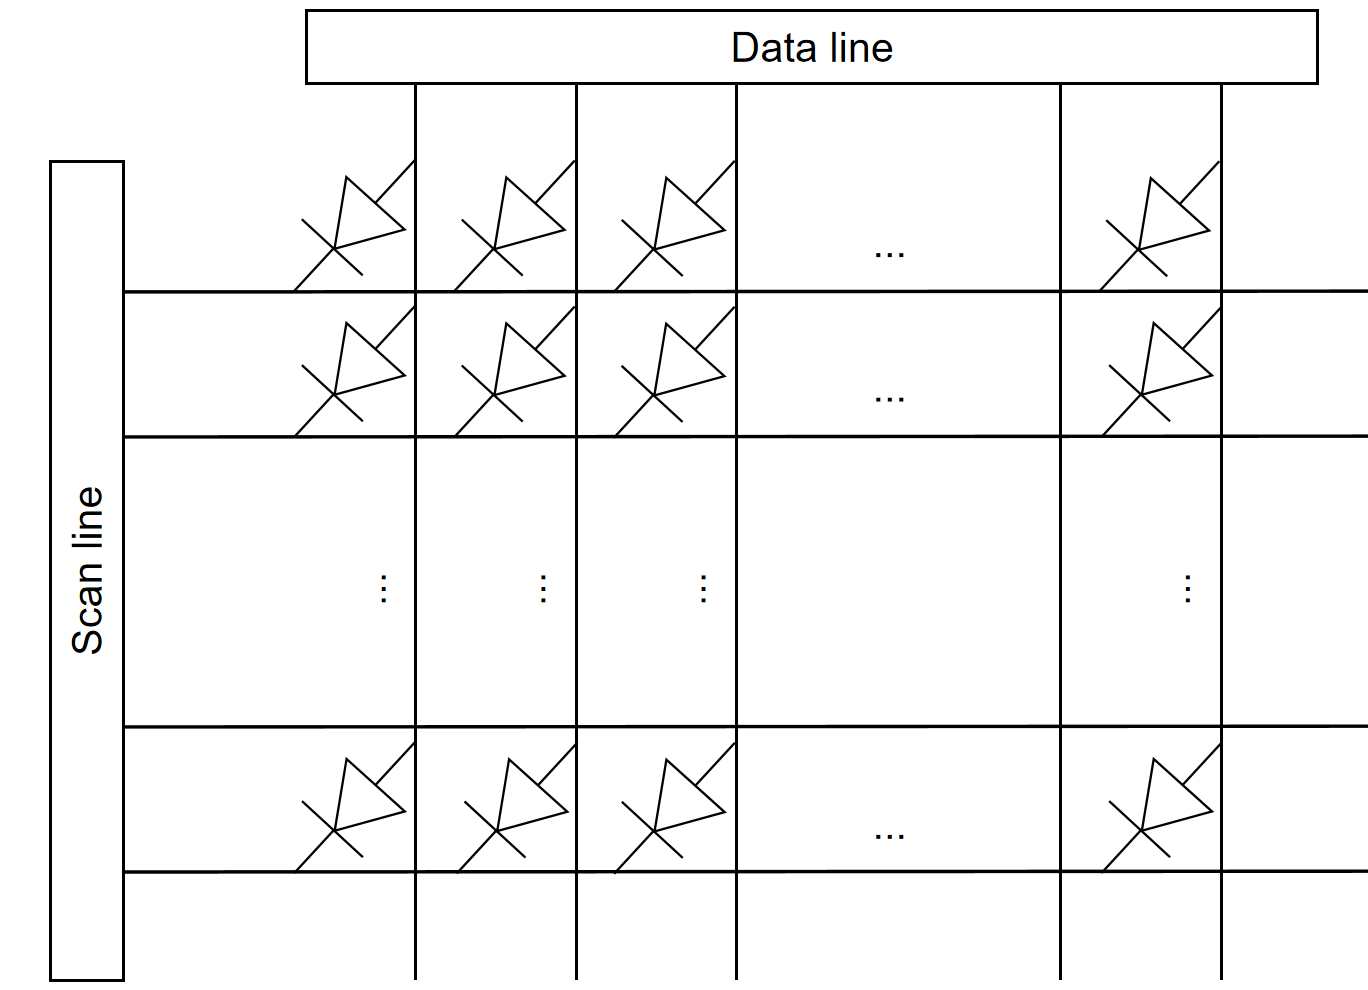
\includegraphics[width=\linewidth]{图片1.1.png}
		\caption{无源驱动等效电路}
        \label{无源驱动等效电路}
	\end{minipage} \hfill
	\begin{minipage}{0.48\linewidth}
		\centering
		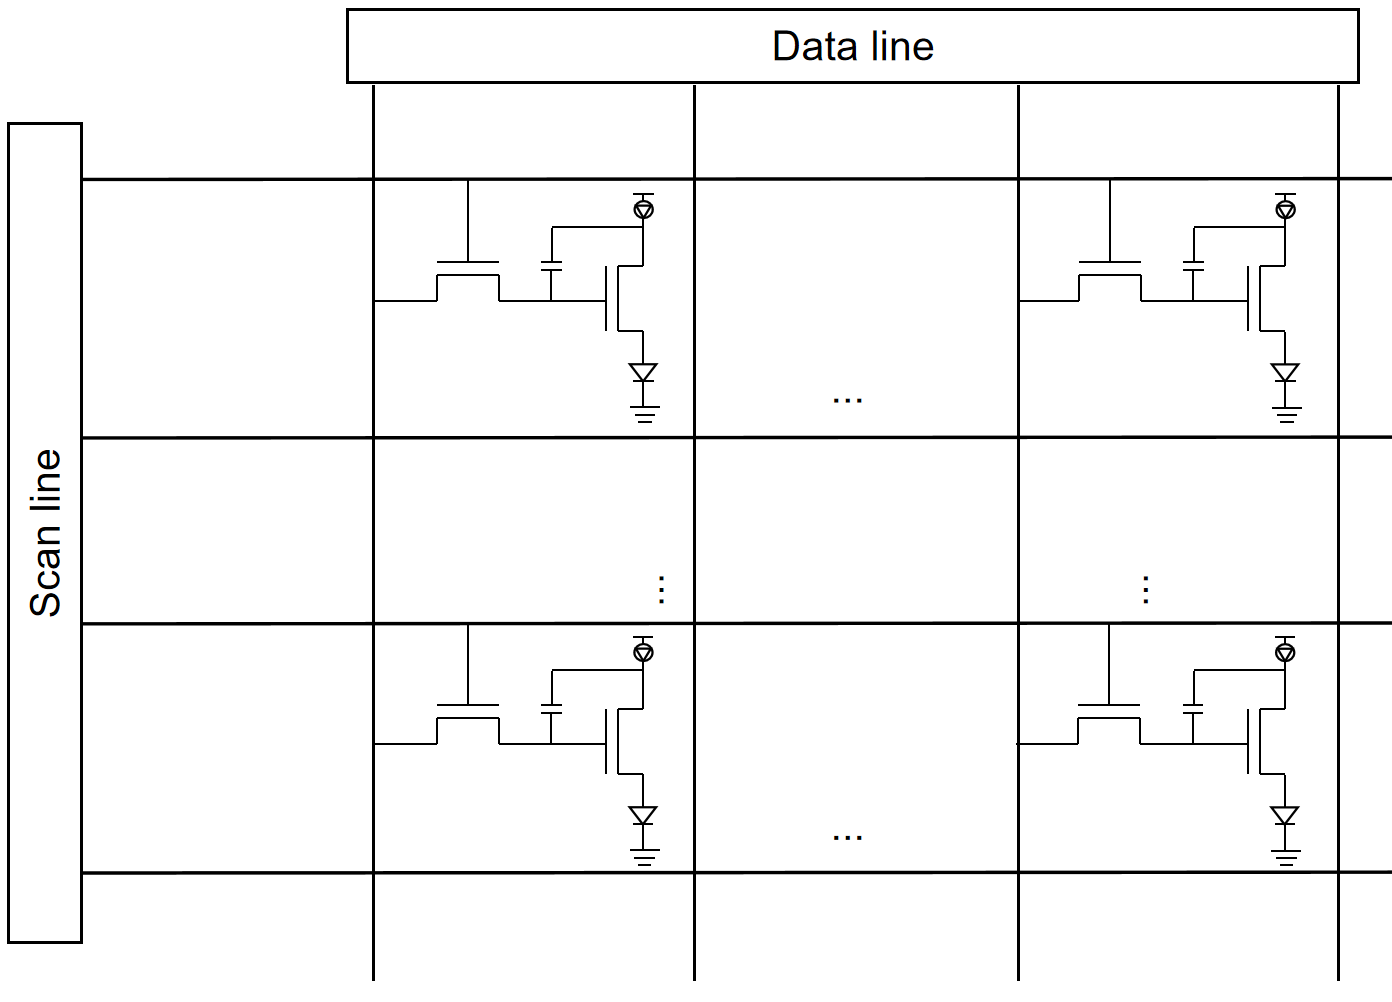
\includegraphics[width=\linewidth]{图片1.2.png}
		\caption{有源驱动等效电路}
        \label{有源驱动等效电路}
	\end{minipage}
\end{figure}

被动矩阵通过行列电极交叉选通，逐行扫描时列电极施加信号使交点像素发光，但其致命缺陷是“交叉效应”——非选通像素在扫描过程中可能承受反向电压，导致漏电流和亮度不均，且发光占空比随分辨率提升显著下降\cite{aliev2002image}，仅适用于低分辨率小尺寸场景（如穿戴设备副屏）。

主动矩阵则为每个像素配备独立的驱动电路（典型如2T1C或更复杂的补偿型架构）\cite{lee20211280}，核心原理是通过扫描线（栅极信号）选通驱动管，将数据电压写入存储电容，由驱动晶体管根据电容电压输出恒定电流至Micro-LED，使其持续发光直至下一帧刷新。这种架构下，发光占空比接近100\%，彻底解决交叉效应，支持高分辨率（如手机屏2K/4K）和大尺寸显示（如电视、户外大屏）。

\section{Micro-LED驱动的研究背景及现状}

\subsection{Micro-LED驱动的研究背景}

Micro-LED是指尺寸在微米级别的发光二极管。与传统LED相比，Micro-LED具有更高的亮度和效率，能够在小尺寸下实现高分辨率的显示效果。其工作原理基于半导体PN结的电致发光效应，通过在GaN基材料中形成PN结，实现电子与空穴的复合发光\cite{蒋府龙2020氮化镓基}。GaN材料的禁带宽度较大，能够发出蓝光和紫外光，通过量子阱结构的设计和优化，可以实现不同波长的发光，满足全彩显示的需求。

尽管Micro-LED在显示性能上具有显著优势，但要实现其在各种应用场景中的高效稳定运行，LED与驱动电路的集成至关重要。在传统的Micro-LED显示系统中，驱动电路通常采用外接驱动芯片，通过邦定等方式与Micro-LED阵列连接\cite{rahman2024tunnel}。近年来，GaN基晶体管凭借其击穿电压大、工作速度快、功耗低、高温持续时间长等优点，在功率开关和射频应用中得到了广泛的研究。这使得同为GaN材料的Micro-LED与驱动晶体管单片集成成为可能。这种单片集成的系统相比于传统驱动方式有着诸多优势，包括更快的开关响应速度，接触电阻和寄生电容更小，高集成度使得设备更加小型化，并且能有效降低总统成本\cite{lu2016monolithic}。

\subsection{国内外研究现状}

Micro-LED的驱动方式一般有两种模式：无源驱动与有源驱动。由于无源驱动采用扫描的方式，每一个时刻内仅有一行像素在发光，占空比非常小，因此不适合大尺寸显示。而采用有源驱动方式时各像素独立可控，是如今研究的主要方向\cite{周律2022micro}。在有源驱动中，TFT（薄膜晶体管）因其电流驱动性较弱及响应速度慢\cite{朱宇轩2024AM-MicroLED显示驱动技术}，同时难以满足高像素密度（ppi）的缺点，因此已经不能满足当今显示器高刷新率以及超高分辨率的需求。而CMOS（互补金属氧化物半导体）驱动具有集成电路超高集成度的特性，通过将Micro-LED与CMOS进行集成可大幅减小电路尺寸与体积。虽然CMOS的优势明显，可以进一步发挥出Micro-LED超小尺寸和超高分辨率的优势，但也存在一定问题，如制备流程较为复杂等\cite{steudel202438}。

在传统的CMOS驱动技术中,通常采用键合和巨量转移的技术将Micro-LED单元和CMOS驱动背板组合在一起，RGB三色Micro-LED器件和CMOS驱动电路器件需要单独进行转移，也就是至少需要转移四次，这无疑使得转移过程更加难以进行，并且还需要进一步处理使CMOS驱动电路与Micro-LED建立连接\cite{周律2022micro}。所以，将驱动的晶体管与LED器件集成在一起，不仅器件性能和可靠性更好，还可以大幅简化制造流程，降低成本。

国内在此领域以及取得了一定成果。2022年福州大学S. Hao等人模拟了一种新型的发光三极管\cite{hao2022fully}。将一个GaN基LED与一个NPN型BJT垂直集成在同一芯片上，其中LED的阴极和BJT的集电极共享同一个N-GaN层。虽然BJT能够实现良好的驱动和调光控制，但其集成结构的制造非常复杂，需要特殊的生长工艺和微加工技术支持，这大大增加了制造成本，降低了成品率，在此体现出了MOSFET作为驱动集成的优势。

在MOSFET驱动集成的研究上，一些高校在这方面起步较早。2014年，台湾师范大学的一个研究小组在暴露的GaN层上制造了MOSFET结构，并串联了LED\cite{huang2015enhanced}。采用MOCVD在蓝宝石衬底上生长了LED结构。然后通过干式蚀刻（ICP）选择性地去除LED结构，以暴露N型GaN层，用于后续的MOSFET制造，然后，在MOSFET表面上的N型GaN层通过标准光刻和ICP干式蚀刻进行图像化，以获得150\,nm的电流通道膜。单片集成MOSFET器件展示了出色的电流注入能力，并能够通过控制栅极电压来调制LED的亮度。

内地高校的研究很快也得到了一定的成果。2016年，华南理工大学的邢陆等人制作了一个将MOSFET与LED相结合的集成器件\cite{lu2017high}。他们在LED顶部生长了P-Gan和N-GaN，实现了P-N-P MOSFET结构。集成器件的I-V特性表明，导通电压为3\,V，导通电阻为4.1\,Ω/cm。在正向注入电流为20\,mA时，LED的电压仅为3.72\,V，器件的光输出功率（LOP）为16\,mW，峰值外量子效率（EQE）高达33\%。

近年随着对GaN MOSFET研究的不断深入，不少团队开始研究如何简化单片集成的制造工艺复杂度。2023年南京大学的庄喆、刘斌团队提出了一种GaN基Micro-LED用准垂直MOSFET驱动的全氮化物单片集成方法\cite{he2024monolithic}，实现了对不同尺寸Micro-LED芯片的电流驱动。GaN基MOSFET具备与氧化物薄膜晶体管类似的电流驱动能力，并且整体集成方案制备难度较低，易与现有芯片结构与制备工艺兼容。2024年国内闽都创新实验室郭太良、严群团队提出了一种新型单片垂直LED-on-FET外延结构\cite{sang2023monolithic}，该集成方案制造过程相对简单，LED和FET之间共享N-GaN层减少了互连电阻并提高了可靠性，同时节省了器件面积，可最大化LED发光区域的开口率并提高阵列器件密度。

目前主流的单片集成方案多采用1T结构，即每个像素由一个晶体管控制LED的开关和亮度。这种方案虽然结构简单、易于实现，但存在电流控制不稳定、动态范围有限等问题。而2T结构通过增加一个晶体管，形成更复杂的驱动电路（如2T1C，即两个晶体管和一个电容），实现电流稳定性提升和动态范围扩展，同时还能有效优化功耗效率。因此2T1C的驱动集成凭借其优异的调控性能，成为研究热点方向之一。

单片集成技术在显示领域发挥着至关重要的作用，相信通过越来越多的研究人员的努力，集成器件的性能将进一步提高，器件结构将更加精简，功能将更加多样化。在不久的将来，片上集成技术在Micro-LED显示领域具有更广阔的应用前景。

\section{研究意义与主要研究内容}

全GaN基Micro-LED的驱动集成研究，核心是解决传统硅（Si）基驱动和非集成方案的 “先天缺陷”，让MicroLED显示技术更高效、可靠地落地。

硅基材料因禁带宽度仅1.12\,eV，在高压高频场景下需复杂电路设计，导致电阻增大、发热严重且信号传输滞后，难以满足Micro-LED阵列的精准驱动需求，同时硅与GaN的晶格失配和热膨胀差异会引发界面应力，造成驱动电路阈值漂移和Micro-LED性能不稳定\cite{selvaraj2018heterogeneous}，影响显示均匀性和寿命。

当前非集成驱动方案依赖外部硅基电路与Micro-LED通过巨量转移键合，这种分离式架构存在连接可靠性差、信号延迟高和功耗大的问题——成千上万的Micro-LED精准贴合焊点难度大，良率低且易接触不良，传输路径的寄生参数导致信号速度受限，无法支持高帧率显示，额外的电平转换电路也增加了能量损耗。全GaN基驱动集成通过将驱动电路与Micro-LED集成于同一个GaN衬底，利用GaN宽禁带（3.4\,eV）和强极化效应，使驱动电路无需复杂结构即可适应高压高频环境，降低电阻和发热，同时同质集成消除了界面应力和缺陷，提升信号传输速度和稳定性\cite{zhu2022improved}。这种集成方式不仅解决了硅基驱动的性能瓶颈和非集成方案的工艺难题，更拓展了Micro-LED在高端显示（如AR/VR）和极端环境中的应用可能，通过简化工艺提升良率并降低成本，是推动Micro-LED从实验室走向产业化的关键技术突破。

本文的主要内容，便是对Micro-LED的驱动电路的集成研究，通过使用Silvaco TCAD仿真软件对Micro-LED的驱动集成电路进行结构仿真，以研究相关特性并加以分析，主要章节安排如下：

第一章为绪论，介绍了Micro-LED的驱动原理，并对Micro-LED驱动的研究背景和现状做了综述，阐明了本文的研究意义。

第二章介绍了仿真所使用的Silvaco TCAD软件，并对仿真参数和模型作出了说明。

第三章介绍GaN基HEMT和MOSFET的工作原理，提出了一种Micro-LED与驱动电路集成的设计方案，并说明了该器件的可行性和优势。

第四章通过对器件仿真得到的相关数据数据进行处理和特性曲线绘制，分析了对结构和器件掺杂进行改变对器件性能的影响，得出相关参数下Micro-LED驱动集成器件的优势所在。


\chapter{仿真软件Silvaco TCAD介绍}

\section{引言}

Silvaco TCAD是由美国Silvaco Inc.开发的专注于半导体器件与工艺仿真的专业EDA工具，该公司自1984年成立以来在该领域积累了超过30年经验，产品覆盖从器件物理到电路设计的全流程仿真，主要服务于半导体制造企业、设计公司、科研机构及高校，用于工艺优化、器件性能预测及新结构研发。

TCAD全称为Technology Computer Aided Design，即计算机辅助设计技术，全球主流TCAD工具包括Silvaco TCAD、Synopsys Sentaurus TCAD、Coventorware等，其中工业界广泛应用于台积电、三星、中芯国际等企业的制程开发，学术界则用于新型器件结构的理论验证。TCAD作为 “虚拟制造” 的核心手段，正通过高效仿真缩短研发周期、减少流片试错成本，成为支撑技术创新与产业竞争力的关键基础设施\cite{fichtner2008overview}。

\section{Silvaco TCAD仿真软件功能组件}

Silvaco TCAD的功能有一维、二维、三维工艺仿真和二维、三维器件仿真。主要组件包括交互式工具Deckbuild、Tonyplot，二维工艺仿真器ATHENA，二维器件仿真器ATLAS，器件编辑器DevEdit和三维仿真器Victory\cite{tang2019silvaco}，此外还有一些内部模块。

\begin{figure}[H]
	\centering
	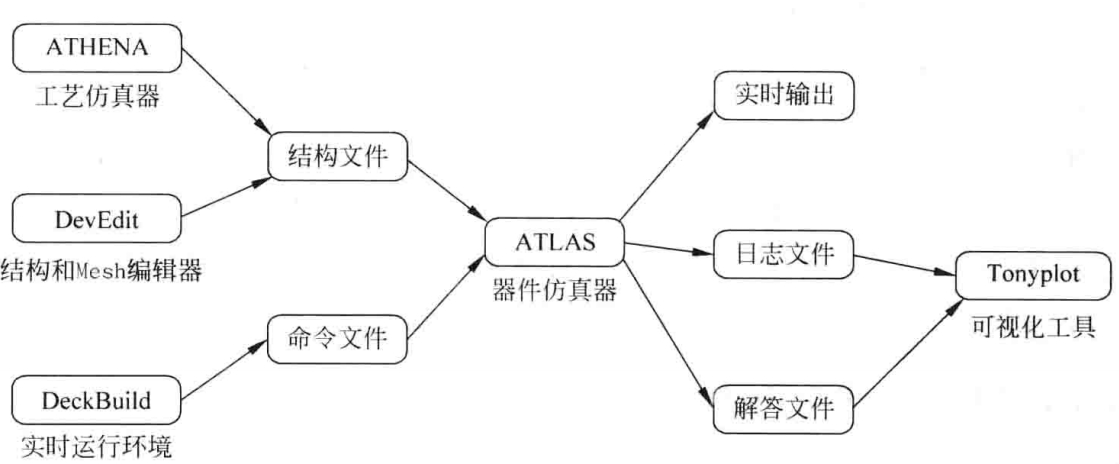
\includegraphics[width=0.75\linewidth]{图片3.1.png}
	\caption{Silvaco TCAD仿真流程}
    \label{Silvaco TCAD仿真流程}
\end{figure}

Silvaco TCAD的仿真流程如图图\ref{Silvaco TCAD仿真流程}所示，由工艺仿真器或器件编辑器得到器件结构，然后通过器件仿真器求解相应的特性，结果由可视化工具Tonyplot显示出来或者显示在实时输出窗口。命令文件的输入和各仿真器的调用都是在集成环境Deckbuild中完成的。本文在研究工作中主要使用了Deckbuild、ATLAS和Tonyplot组件。

Deckbuild是一个交互式的、图形化的实时运行环境，在工艺和器件仿真中作为仿真平台。其界面如图\ref{Deckbuild交互界面}所示：

\begin{figure}[H]
	\centering
	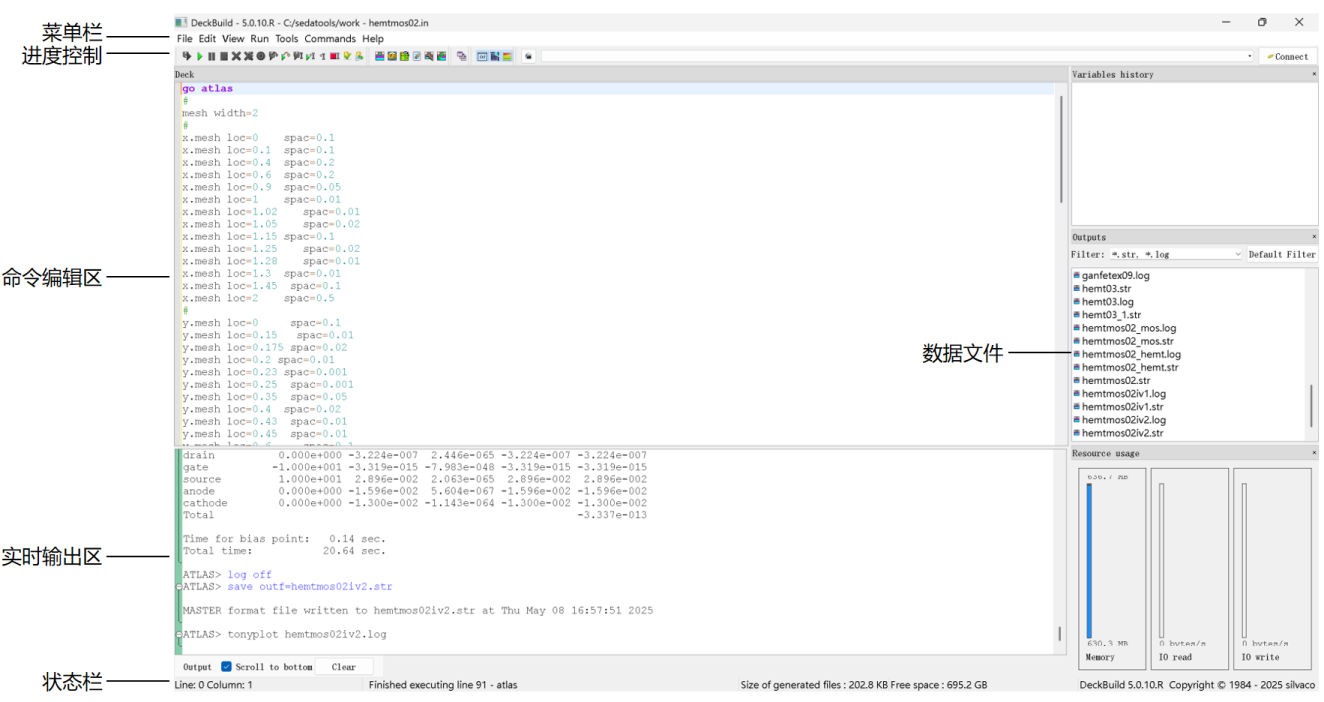
\includegraphics[width=\linewidth]{图片3.2.png}
	\caption{Deckbuild交互界面}
    \label{Deckbuild交互界面}
\end{figure}

Deckbuild的顶部是菜单栏和进度控制，菜单栏中包括新建、打开、撤销等常用编辑操作，进度控制中包含开始运行、设置断点、结束运行等操作。Deckbuild的上部为命令编辑区，下部为实时输出区，底部和右部下方则为软件运行状态显示栏，右部中间位置则为输出文件显示区，代码运行时生成的文件会显示在这里。

ATLAS器件仿真器可以仿真半导体器件中的电学、光学和热学行为。ATLAS提供一个基于物理的、使用简便的、模块化的、可拓展的平台，用以分析二维和三维模式下半导体器件的直流、交流和时域响应。ATLAS可以仿真硅化物、Ⅲ-Ⅴ族化合物或聚合有机物等材料，还可以仿真CMOS、LED或者HEMT等器件\cite{1014325203.nh}。在本文的研究中将使用ATLAS仿真HEMT和MOS器件。

ATLAS的仿真是通过对一系列状态的描述来进行组织的，而这些状态可以分为结构生成、设定材料模型、计算方法、器件特性获取和结果分析五组状态。在结构生成时，用户可以自定义材料的参数，如迁移率参数、寿命参数、能带参数和介电常数等，也可以自定义材料，ATLAS会根据用户输入的参数调整物理模型的参数值。材料模型和计算方法将会在本章的剩余小节介绍。点击进度控制栏上的运行按钮，ATLAS会根据参数和模型计算出器件的特性，并输出用户想要的结果。

Tonyplot是一个可视化工具，可以将仿真生成的结构文件（.str）、器件仿真保存的log文件（.log）和提取到的dat文件（.dat）显示出来。同时Tonyplot也是一个交互式的工具，可以通过cutline功能对一定长度线段上的物理量进行显示。在本文中将大量使用Tonyplot的显示和cutline功能，以得到器件的能带、载流子浓度和电学特性曲线等数据。

\section{模型介绍}

在半导体器件仿真中，合理选择物理模型是准确预测器件电学特性的关键。本研究基于Silvaco TCAD仿真平台，针对器件内部载流子的复合、输运及极化效应等物理过程，选取了srh复合模型、conmob迁移率模型、albrct温度相关迁移率模型及极化效应模型，通过多模型协同仿真实现对器件行为的定量描述,相关代码如图\ref{Deckbuild中的模型设置命令代码}所示。

\begin{figure}[H]
	\centering
	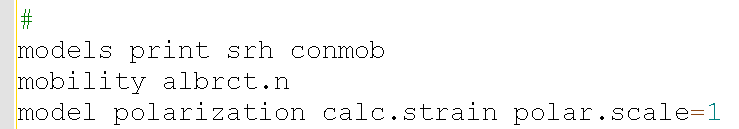
\includegraphics[width=\linewidth]{图片3.3.png}
	\caption{Deckbuild中的模型设置命令代码}
    \label{Deckbuild中的模型设置命令代码}
\end{figure}

models print srh conmob语句中print是Silvaco TCAD的软件参数，用以在Deckbuild的输出窗口列出仿真模型及参数。

srh是Shockley-Read-Hall复合模型，用于描述半导体中通过杂质或缺陷能级（陷阱）发生的间接载流子复合过程，这是非平衡载流子复合的主要机制之一\cite{HighSpeedSemiconductorDevices}。其核心思想是：电子和空穴通过陷阱能级实现能量与动量的交换，复合率由陷阱浓度、载流子浓度及陷阱能级位置共同决定。数学表达式为：
\begin{equation}
R_{SRH} = \frac{n \cdot p - n_i^2}{\tau_p(n + n_1) + \tau_n(p + p_1)}
\end{equation}
式中，n和p分别为电子和空穴的实际浓度，\(n_i\)是本征载流子浓度（由材料禁带宽度和温度决定），\(\tau_n\)和\(\tau_p\)分别表示电子和空穴的寿命（反映陷阱对载流子的捕获能力），\(n_1\)和\(p_1\)是与陷阱能级位置相关的常数（当陷阱能级位于禁带中央时，\(n_1 = p_1 = n_i\)）。该模型通过引入陷阱相关参数，能够准确模拟器件中因缺陷或界面态引起的载流子复合效应，尤其适用于分析掺杂半导体或异质结界面的复合行为，非常适合本研究中对于GaN基HEMT和MOSFET中AlGaN和GaN界面的情况。

Conmob是浓度依赖迁移率模型，载流子迁移率是决定器件导电能力的关键参数，而掺杂浓度直接影响迁移率大小——高掺杂时，电离杂质散射加剧，迁移率下降\cite{HighFieldTransportSemiconductors}。Conmob模型通过分段函数形式，定量描述迁移率随掺杂浓度的变化规律，其表达式为：
\begin{equation}
\mu(N) = \mu_{\text{min}} + \frac{\mu_{\text{max}} - \mu_{\text{min}}}{1 + \left(\frac{N}{N_{\text{ref}}}\right)^\alpha}
\end{equation}
其中，\(\mu(N)\)为当前掺杂浓度N下的迁移率，\(\mu_{\text{max}}\)和\(\mu_{\text{min}}\)分别表示低掺杂极限迁移率和高掺杂极限迁移率（由材料晶格散射和杂质散射特性决定），\(N_{\text{ref}}\)是迁移率开始显著下降的参考浓度，\(\alpha\)为拟合参数（反映迁移率随浓度变化的敏感程度）。该模型通过实验数据拟合确定参数，能够有效刻画硅基半导体中电子和空穴迁移率随掺杂浓度的变化趋势，是器件电导特性仿真的基础模型之一。

mobility albrct.n 语句中的albrct是温度依赖性迁移率修正，温度对载流子迁移率的影响主要体现在晶格散射效应上——温度升高时，晶格振动加剧，载流子与声子的碰撞概率增加，迁移率随温度呈负指数关系下降。Albrct 模型通过引入温度修正项，对迁移率的温度依赖性进行描述。

model polarization calc.strain polar.scale=1语句是极化效应模型参数的命令，在III-V族等极性半导体异质结中，自发极化和压电极化会在界面处积累大量极化电荷，形成高浓度二维电子气（2DEG），显著影响器件导电特性\cite{zhou2020polarization}。因此需要极化效应模型通过计算材料应变与极化强度的耦合关系，引入附加电荷密度：
\begin{equation}
\Delta\rho_{\text{pol}} = \nabla \cdot \mathbf{P}_{\text{total}}
\end{equation}
其中，总极化强度\(\mathbf{P}_{\text{total}}\)包括自发极化\(\mathbf{P}_{\text{spont}}\)（由晶体结构对称性决定，如 AlGaN 材料的固有极化特性）和压电极化\(\mathbf{P}_{\text{piezo}}\)（由晶格失配引起的应变产生，表达式为\(\mathbf{P}_{\text{piezo}} = e_{ij} \cdot \varepsilon_{jk}\)，\(e_{ij}\)为压电张量，\(\varepsilon_{jk}\)为应变张量）。仿真中通过calc.strain选项激活应变计算，并利用polar.scale参数调整极化效应的比例系数，以适配不同异质结结构（如AlGaN/GaN异质结）的界面电荷分布模拟，准确反映极化效应对器件阈值电压、导电沟道浓度的影响。

上述模型的联合应用，能够从载流子复合、输运及界面电荷调控等多个维度，刻画半导体器件内部的物理过程。在GaN基的HEMT和MOSFET仿真中，srh模型用于分析缺陷引起的漏电流，conmob和albrct模型描述沟道载流子迁移率的浓度与温度依赖性，极化模型则定量计算界面2DEG的形成机制。通过参数校准与多物理场耦合，可实现对器件I-V特性、温度稳定性及界面效应的精准预测，为器件结构优化和工艺参数设计提供理论支撑\cite{wong2023tcad}\cite{munir2006epilayer}。

\section{数值计算方法}

Silvaco TCAD 作为半导体器件仿真的核心工具，其数值计算方法直接决定了仿真的精度与效率。这些方法基于半导体物理方程构建，通过离散化和迭代求解实现对器件物理行为的精确模拟。

离散化包含两重含义：一是通过建立网络使连续的结构离散化，二是基本物理方程算法中物理量的离散化。其中第一点需要使用者在Deckbuild中编写命令代码划分器件的横向和纵向网格线，在界面接触处需要密集以提升仿真精度，在材料层中部则需要稀疏以减少不必要的仿真器性能消耗，如图\ref{HEMT器件结构中的网格划分}所示：

\begin{figure}[H]
	\centering
	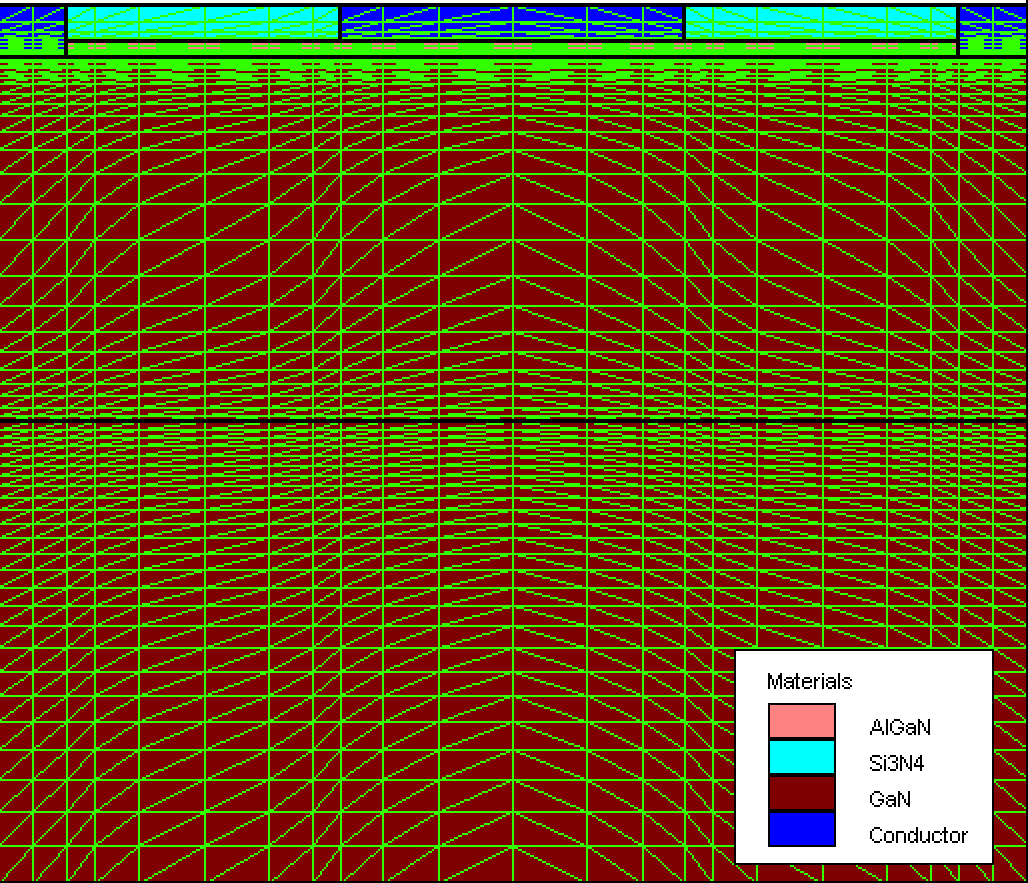
\includegraphics[width=0.5\linewidth]{图片3.4.png}
	\caption{HEMT器件结构中的网格划分}
    \label{HEMT器件结构中的网格划分}
\end{figure}

第二点则是ATLAS仿真器对基本物理方程的离散化，在仿真过程中，半导体器件的物理行为通过求解泊松方程、电子连续性方程和空穴连续性方程来描述，这些偏微分方程需通过数值方法如有限差分法（Finite Difference Method,FDM）或有限元法（Finite Element Method,FEM）进行离散化处理为代数方程组以实现数值求解。

为了求解上述方程，ATLAS使用了newton迭代法来求解。牛顿迭代法是求解非线性方程组的经典数值方法，其核心思想是通过逐次线性化将非线性问题转化为线性问题求解。对于非线性方程 \(F(x) = 0\)，假设当前迭代点为 \(x^k\)，在该点处对 \(F(x)\) 进行泰勒展开并保留一阶项：\(F(x^{k+1}) \approx F(x^k) + J(x^k)(x^{k+1} - x^k) = 0\)其中，\(J(x^k)\) 为雅可比矩阵（Jacobian Matrix），描述 \(F(x)\) 在 \(x^k\) 处的梯度信息。通过求解线性方程组：\(J(x^k) \Delta x^k = -F(x^k)\)得到迭代步长 \(\Delta x^k = x^{k+1} - x^k\)，进而更新解向量 \(x^{k+1} = x^k + \Delta x^k\)。重复此过程直至残差 \(||F(x^k)||\) 小于设定阈值（如 \(10^{-12}\)），实现对非线性方程的收敛求解。

在由泊松方程、电子/空穴连续性方程等强非线性偏微分方程组的求解中，非常适合使用newton迭代法来求解，因此Silvaco TCAD的ATLAS仿真器将其采用为默认求解方法。

\section{本章小结}

本章详细介绍了用于研究的Silvaco TCAD仿真软件。该软件由美国Silvaco Inc.开发，在半导体领域应用广泛，其Deckbuild、ATLAS和Tonyplot组件分别负责提供仿真平台、模拟器件行为和可视化数据。为准确模拟器件特性，研究选用了srh复合、conmob迁移率、albrct温度相关迁移率及极化效应等模型，从多维度描述器件内部物理过程。Silvaco TCAD采用离散化处理和牛顿迭代法求解方程，保障了仿真的精度和效率，为后续研究Micro-LED驱动集成器件的特性奠定了坚实基础。


\chapter{Micro-LED驱动集成器件结构设计}

\section{引言}

在Micro-LED主动矩阵显示技术中，驱动电路的核心是通过晶体管阵列实现像素级电流控制。传统硅基驱动方案因材料兼容性差、高频损耗大等问题，难以满足Micro-LED对微安级电流精度和高速响应的需求。针对这一挑战，本章提出一种全GaN基HEMT与MOSFET集成驱动器件结构，利用GaN材料的宽禁带特性与极化效应，实现开关管（HEMT）与驱动管（MOSFET）的单片集成，为Micro-LED阵列提供高效、稳定的电流驱动解决方案。

\section{GaN基HEMT和MOSFET的工作原理}

GaNHEMT为异质结结构器件，通过在GaN层上气相淀积或分子束外延生长AlGaN层，形成AlGaN/GaN异质结。当无外加应力条件时，GaN晶体内的正负电荷中心发生分离，在沿极轴的方向上产生极化现象，这种现象称为GaN的自发极化效应\cite{1017297259.nh}。在外加应力下，由于晶体受到应力产生晶格形变，使得内部正负电荷发生分离，在晶体内部形成电场，导致晶体表面感应出极化电荷，发生压电效应。由于压电极化和自发极化电场方向相同，在电场作用下使得异质结界面交界处感应出极化电荷\cite{parikh2003algan}。

由于AlGaN材料具有比GaN材料更宽的带隙，在到达平衡时，异质结界面交界处能带发生弯曲，造成导带和价带的不连续，在异质结界面形成一个三角形的势阱。从图\ref{HEMT能带图}中可以看到，在GaN一侧，导带底E\textsubscript{c}已经低于费米能级E\textsubscript{f}，所以会有大量的电子积聚在三角形势阱中。同时宽带隙AlGaN一侧的高势垒，使得电子很难逾越至势阱外，电子被限制横向运动于界面的薄层中，这个薄层被称之为二维电子气(2DEG)\cite{1017297259.nh}。

\begin{figure}[H]
	\centering
	\begin{minipage}{0.48\linewidth}
		\centering
		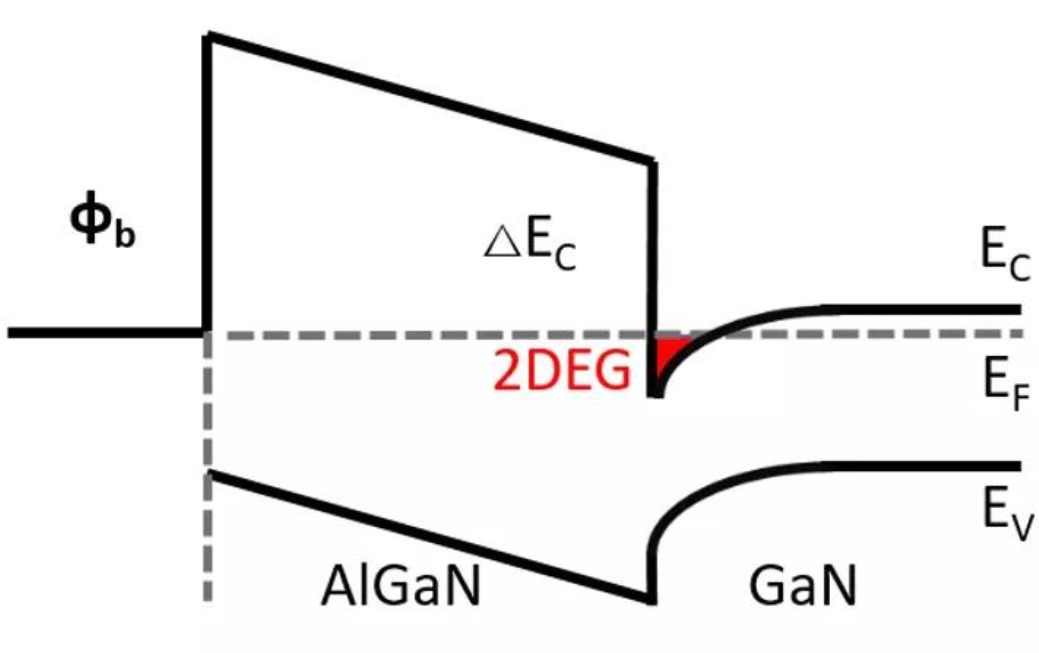
\includegraphics[width=\linewidth]{图片1.3.png}
		\caption{HEMT能带图}
        \label{HEMT能带图}
	\end{minipage} \hfill
	\begin{minipage}{0.48\linewidth}
		\centering
		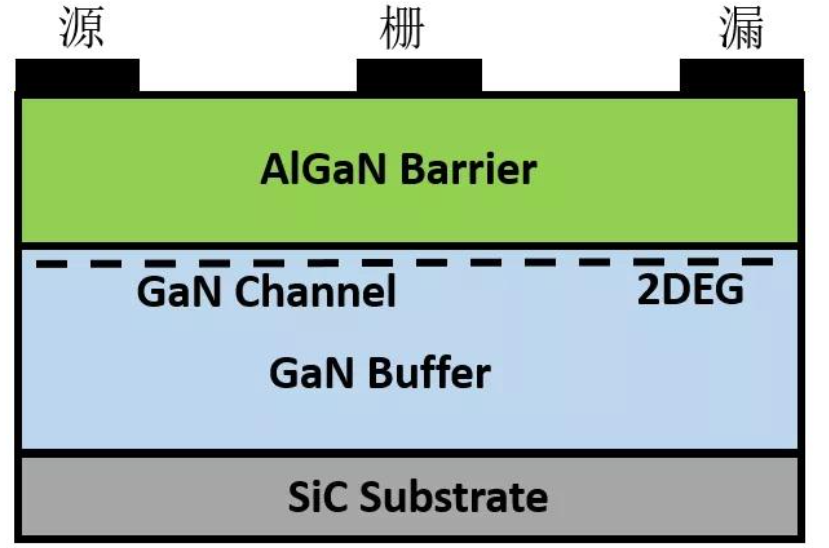
\includegraphics[width=\linewidth]{图片1.4.png}
		\caption{HEMT结构示意图}
        \label{HEMT结构示意图}
	\end{minipage}
\end{figure}

AlGaN/GaN HEMT器件结构如图图\ref{HEMT结构示意图}所示。漏源电压V\textsubscript{ds}使得沟道内产生横向电场，在横向电场作用下，二维电子气沿异质结界面进行输运形成漏极输出电流I\textsubscript{ds}。栅极与AlGaN势垒层进行肖特基接触，通过栅极电压V\textsubscript{gs}的大小控制AlGaN/GaN异质结中势阱的深度，改变沟道中二维电子气面密度的大小，从而控制沟道内的漏极输出电流。

GaN基MOSFET（金属氧化物半导体场效应晶体管）的工作原理基于栅极电场对半导体表面载流子的调控，其核心机制与传统硅基MOSFET类似，但因GaN材料的宽禁带特性（3.4\,eV）和异质结设计而具备更高的电压耐受性和效率\cite{mehta2015gan}。

增强型GaN MOSFET的阈值电压（V\textsubscript{th}）由栅氧化层厚度、材料功函数及界面态密度决定。零栅压时，GaN表面呈高阻态；施加正栅压后，电场穿透氧化层，吸引GaN中的电子在表面形成N型反型沟道，连接源漏极实现导通\cite{meneghini2021gan}。

GaN基的HEMT和MOSFET两者均受益于GaN的宽禁带特性，在高压、高频、高温场景中展现出硅基器件难以企及的优势\cite{wuerfl2011reliability}。

\section{驱动电路工作原理}

本文设计的GaN基Micro-LED驱动集成器件基于经典2T1C（两晶体管一电容）矩阵架构，通过右侧驱动晶体管与左侧开关晶体管的协同工作，实现对Micro-LED像素的灰度控制与稳定电流驱动，其电路等效原理图如图\ref{驱动器件工作电路原理图}所示：

\begin{figure}[H]
	\centering
	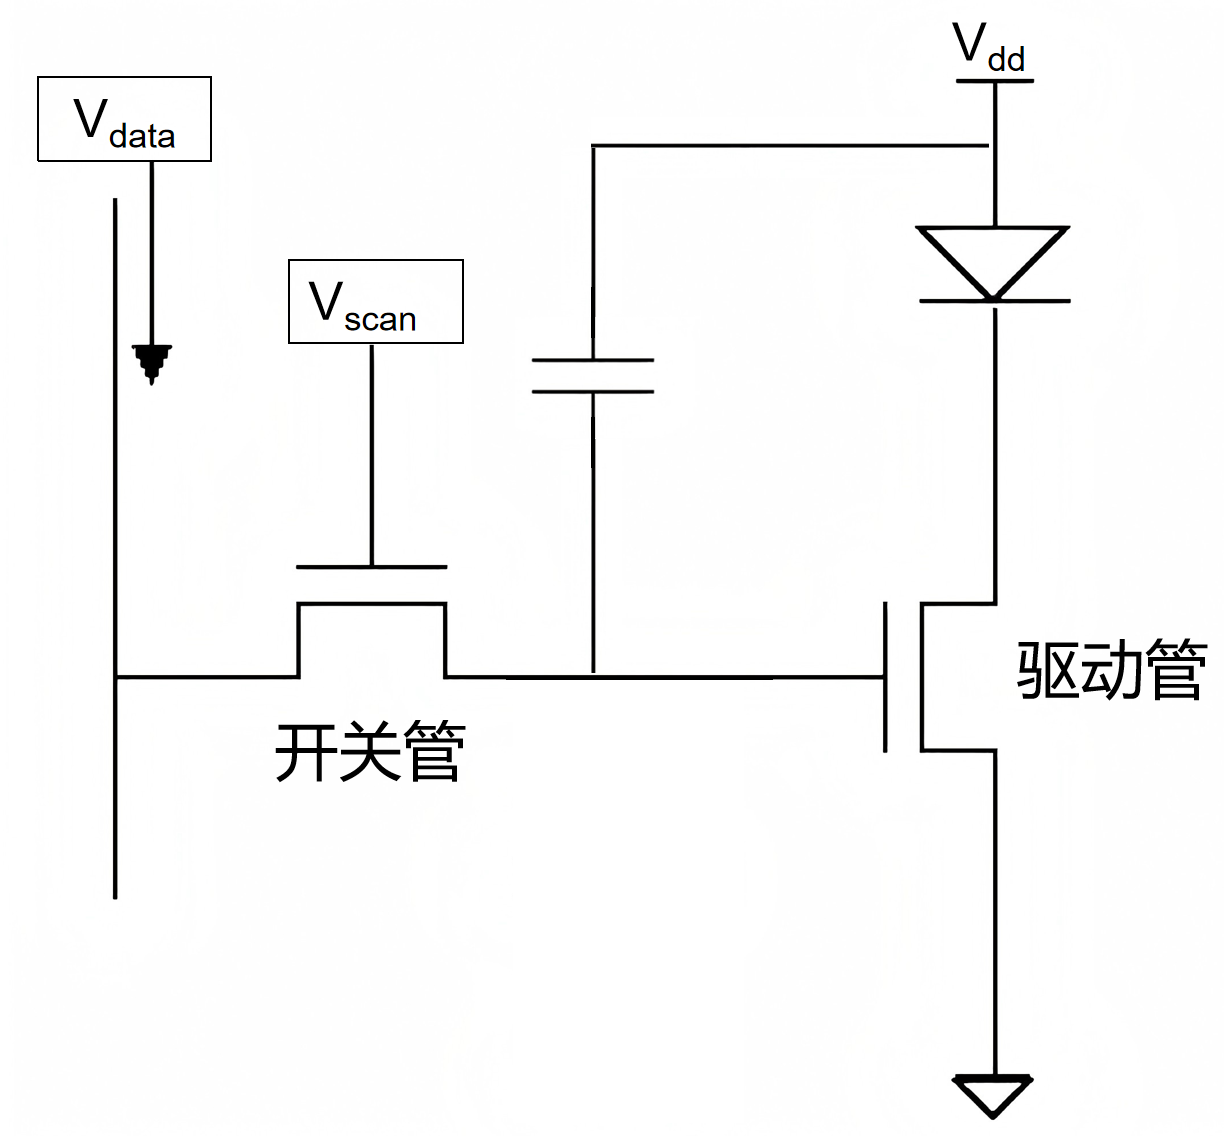
\includegraphics[width=0.5\linewidth]{图片2.2.png}
	\caption{驱动器件工作电路原理图}
    \label{驱动器件工作电路原理图}
\end{figure}

整个工作过程可分为信号写入、电流保持与动态驱动三个连续阶段：
\begin{enumerate}
    \item 信号写入阶段（扫描线高电平时期）：当扫描线（V\textsubscript{scan}）施加高电平信号时，右侧开关管栅极电压即为V\textsubscript{scan}，使其进入导通态。此时，数据电压（V\textsubscript{data}）通过列电极施加至开关管的漏极，经导通通道向存储电容充电。存储电容的下极板与驱动管的栅极以及开关管源极相连，因此电容电压V\textsubscript{c}迅速跟随V\textsubscript{data}电压变化，完成像素灰度信号的临时存储。这一过程中，驱动管需要具有高电子迁移率与低导通电阻确保了数据信号的快速写入，以满足高刷新率的时序要求。
    \item 电流保持阶段（扫描线低电平时期）：扫描线电压降至低电平后，开关管进入截止态，切断数据电压与存储电容的连接。此时，存储电容维持的电压V\textsubscript{c}施加于右侧驱动管的栅极，使驱动管保持导通状态。驱动管需要具有高开关比与低漏电流以确保了电容电压在一帧周期内的衰减极小甚至忽略不计，从而维持稳定的栅极驱动信号，直至下一个周期的V\textsubscript{scan}。
    \item 动态驱动阶段（驱动管电流输出过程）：导通的驱动管作为电流通路，将存储电容的电压信号转换为驱动电流。此时，Micro-LED的阳极连接至电源（V\textsubscript{dd}），阴极通过驱动管的漏极与源极接地。漏极电流I\textsubscript{ds}通过驱动管的栅极电压在一定范围内调节，直接驱动Micro-LED像素发光，亮度与I\textsubscript{ds}呈正比例关系。
\end{enumerate}

2T1C驱动架构的协同核心在于 “电压存储—电流输出” 的信号转换：驱动晶体管作为高速写入器，负责将数据电压精准写入存储电容；开关晶体管作为恒流开关，将电压信号转换为稳定电流。

\section{整体架构与双晶体管集成方案}

本文设计的驱动集成器件采用“HEMT+MOSFET双晶体管共衬底集成架构”，适配主动矩阵显示的2T1C（两晶体管一电容）经典驱动电路。器件结构以GaN为统一衬底，左侧为耗尽型GaN HEMT（开关管），右侧为增强型GaN MOSFET（驱动管），两者通过共享n型GaN层实现电流路径耦合，结构从下至上依次如图\ref{驱动集成器件结构示意图}所示：

\begin{figure}[H]
	\centering
	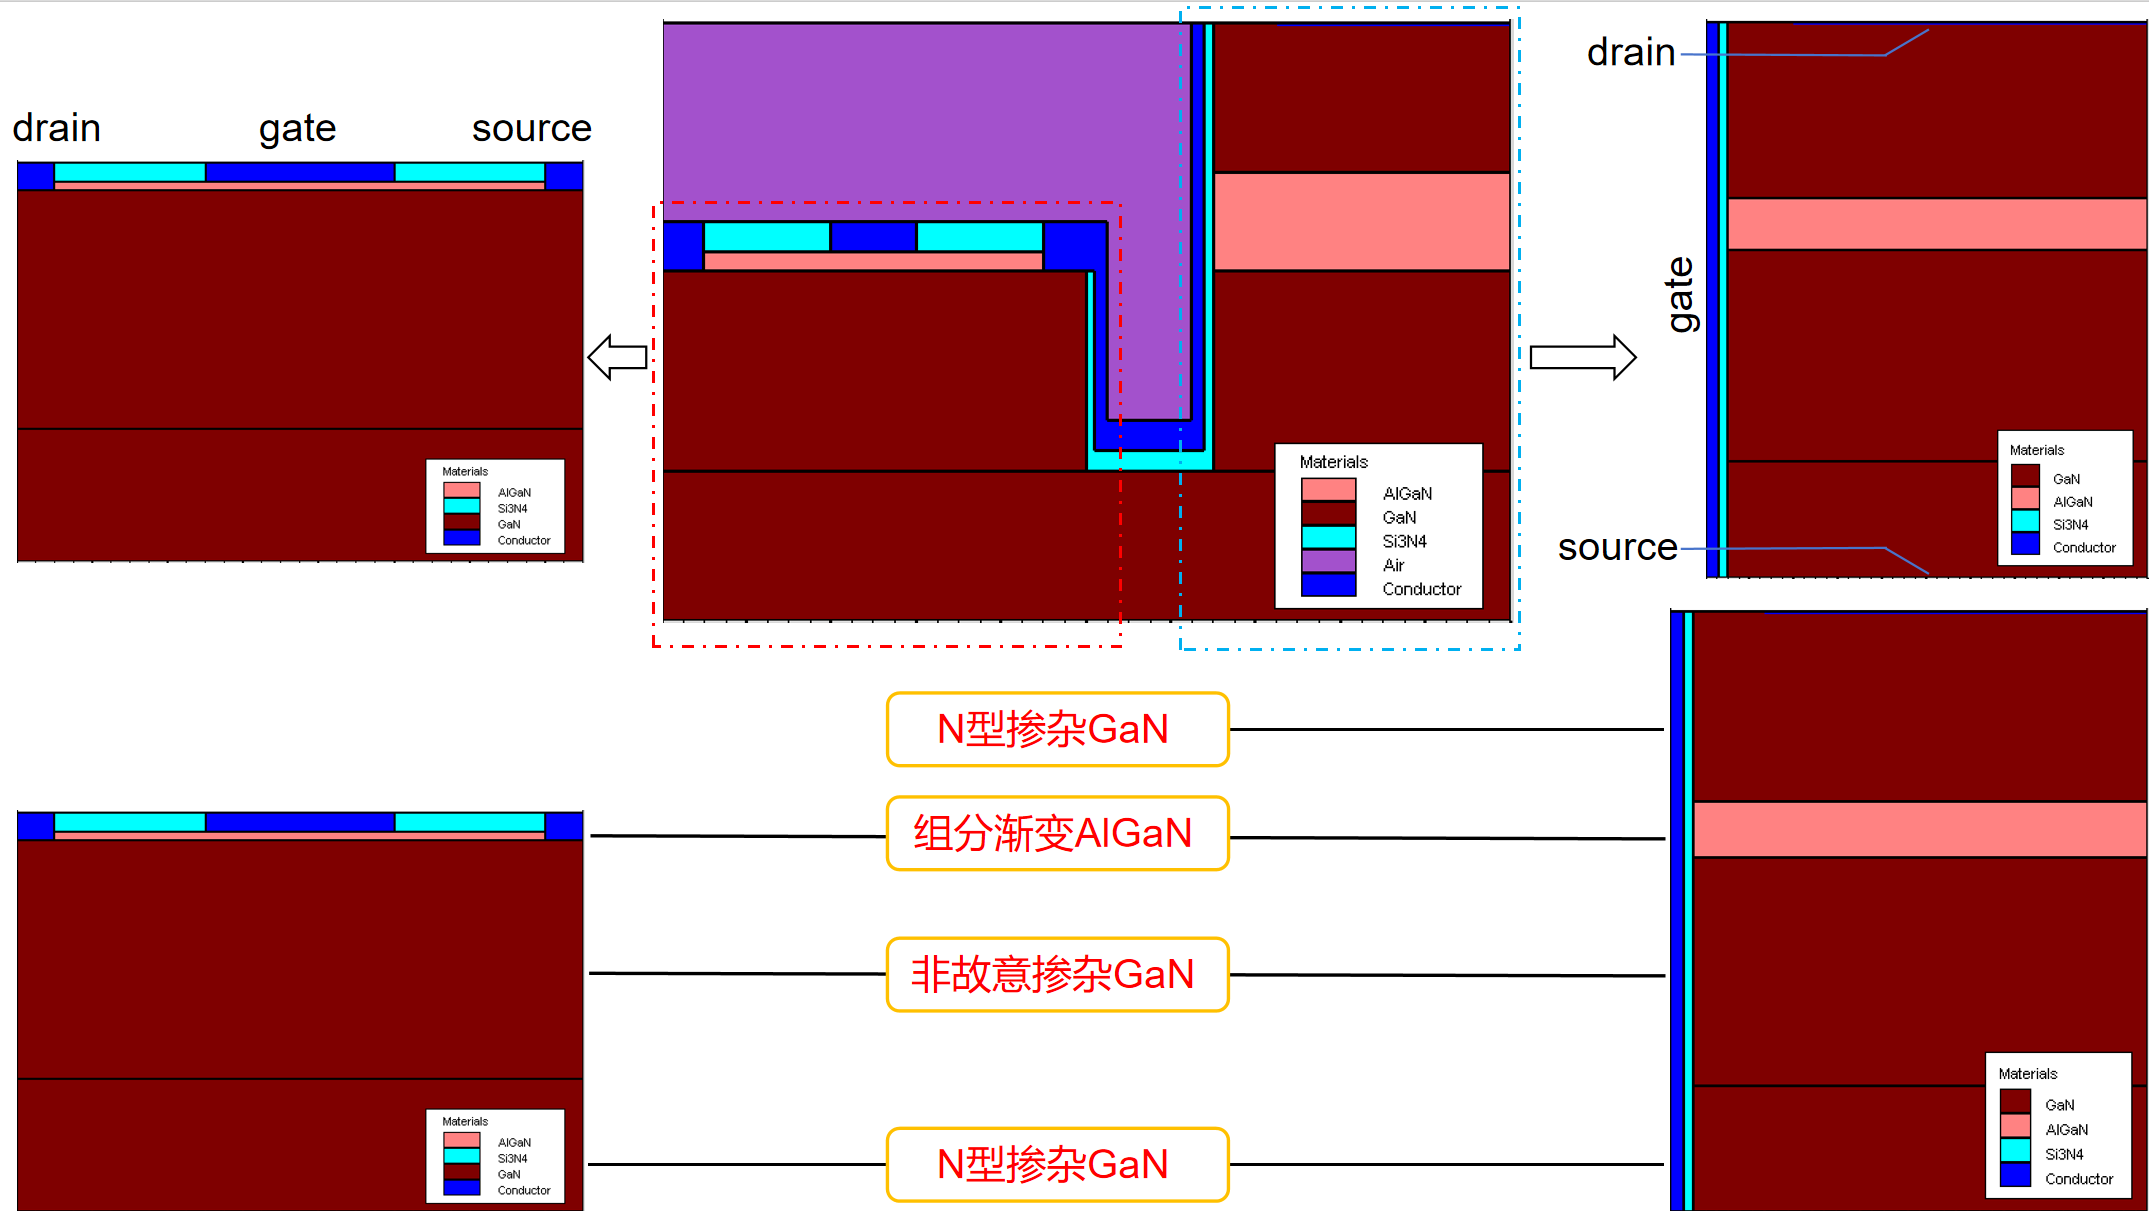
\includegraphics[width=\linewidth]{图片2.1.png}
	\caption{驱动集成器件结构示意图}
    \label{驱动集成器件结构示意图}
\end{figure}

器件最底层为N型掺杂GaN层（图中红色部分），兼具衬底支撑与低阻电流通道功能，其核心优势在于完全消除异质衬底带来的晶格失配与热膨胀差异问题。相较于硅基（晶格失配率17\%）\cite{唐林江2020宽禁带半导体材料}或蓝宝石衬底（失配率14\%）\cite{liu2014stress}，GaN基板与上层外延层的晶格常数几乎一致，可将界面位错密度降低，显著提升器件长期工作的可靠性。同时，GaN本征热导率达230\,W/m·K\cite{mion2006accurate}，能够快速导出驱动过程中产生的热量，为高稳定性电流输出奠定基础。同时，将衬底接地，与MOSFET的源极相连，作为电流的流通通道。

在GaN衬底之上，通过金属有机化学气相沉积（MOCVD）生长非故意掺杂GaN层（图中红色部分），作为缓冲层隔离衬底杂质扩散，同时为AlGaN层生长提供平整界面。

在非故意掺杂的GaN层上生长组分渐变的AlGaN层（图中粉色部分），其铝（Al）组分在AlGaN最下方为0.2，渐变至最上方为0。在左侧的HEMT中，利用AlGaN与GaN的极化效应差异，在AlGaN/非故意掺杂GaN界面累积高密度负电荷，形成二维电子气（2DEG）沟道。在右侧的MOSFET中，铝（Al）组分从底部到顶部线性递减，在AlGaN层内部产生反向压电极化电场，诱导出高密度空穴形成三维空穴气（3DHG）导电层，替代传统Mg掺杂p型GaN。

最上方则为N型掺杂的GaN层（图中红色部分），与下方3DHG层和同为N掺杂的衬底层形成N-P-N结构，作为LED的控制驱动管。

通过电感耦合等离子体刻蚀（ICP）形成HEMT与MOSFET的独立区域，形成器件的主要结构。

再通过原子层沉积（ALD）形成Si\textsubscript{3}N\textsubscript{4}（图中青色部分）作为MOSFET的栅极绝缘层，同时将各电极隔离开以保证工作稳定性。选用Si\textsubscript{3}N\textsubscript{4}作为绝缘层可显著提升GaN基器件性能。其高介电常数与击穿电压能有效隔离器件并约束电场，低晶格失配与热膨胀系数确保界面稳定，兼具掩膜与绝缘功能简化工艺流程，较高热导率助力散热，成熟工艺与低成本优势则适配量产需求，实现器件可靠性与经济性的双重优化。

在绝缘层上再进行光刻开孔等步骤沉积金属电极（图中蓝色部分）。部分电极由于仿真器需要对器件结构进行简化以提升性能，故未设置厚度，在仿真器剖面图中未显示，但在示意图中已标出。在左侧的HEMT中，中间的栅极采用肖特基接触结构，通过栅极电压调控2DEG浓度。在右侧的MOSFET中，栅极为竖置，通过施加电压在AlGaN层中形成导电沟道。

\section{优势分析}

器件的核心优势源于GaN材料体系的同质集成特性、AlGaN渐变组分层的创新设计及2T1C架构的协同优化，从性能、工艺、可靠性多维度突破传统硅基驱动方案的瓶颈。

本文提出的驱动集成器件优化了动态响应性能。在高灰度级场景（如白色像素），V\textsubscript{data}电压较高，HEMT深度导通，存储电容快速充电至V\textsubscript{data}，MOSFET输出最大电流，驱动Micro-LED达到峰值亮度；在低灰度级场景（如黑色像素），V\textsubscript{data}电压较低（略高于MOS的V\textsubscript{th}），MOSFET工作于亚阈值区，实现精细的亮度调节。由于MOSFET在饱和区的漏极电流几乎不随漏源电压（V\textsubscript{ds}）变化（恒流特性），可有效抑制Micro-LED正向电压波动对亮度的影响，这一特性在大尺寸显示阵列中尤为重要。

此外还实现了全层级外延结构的工艺与可靠性突破。器件从衬底到功能层均采用GaN基材料体系，所有外延层级完全相同，彻底消除传统异质集成中的晶格失配与热应力问题。这种设计使AlGaN/GaN异质结界面位错密度较硅基衬底方案降低三个数量级。全层级外延还简化了制备流程，MOCVD生长过程无需中断或更换气源，减少界面污染风险。在高温工作环境下，同质结构的热膨胀系数匹配性避免了层间开裂风险，使器件寿命大幅延长，满足车载显示、工业控制等高可靠性场景需求。

最重要的是使用三维空穴气（3DHG）对P型掺杂GaN的革命性替代。

传统GaN基器件依赖Mg离子实现P型掺杂，但Mg受主在GaN中的激活效率极低（通常 <30\%），且需高温退火以部分激活，这一过程会引入多重负面效应。高浓度Mg掺杂（如Mg离子流率从250\,sccm提升至500\,sccm）会导致P-GaN层中缺陷密度显著增加，形成高密度acceptor-like陷阱（密度达 9.5×10\textsuperscript{19}cm\textsuperscript{-3}）\cite{guo2022influence}，这些陷阱在反向偏压下电离并捕获载流子，导致器件性能严重退化。

Mg掺杂的另一核心问题是高温退火引发的材料损伤。退火过程中Mg离子会强烈扩散至AlGaN/GaN异质结界面，形成补偿中心，导致二维电子气（2DEG）浓度下降15\%-20\%。此外，Mg过载会导致P-GaN层晶体质量恶化，位错密度从低掺杂的10\textsuperscript{6}cm\textsuperscript{-2} 升至10\textsuperscript{8}cm\textsuperscript{-2}，进而使空穴迁移率从20\,cm\textsuperscript{2}/(V·s) 降至10\,cm\textsuperscript{2}/(V·s) 以下，显著增加P型区电阻\cite{guo2022influence}。

本器件通过AlGaN反向渐变组分设计诱导的3DHG，从根本上规避了Mg掺杂的缺陷。3DHG依赖极化效应生成，无需高温激活。更重要的是，3DHG结构消除了Mg离子扩散引起的2DEG浓度波动，从物理机制上解决了P型掺杂带来的可靠性难题。

\section{本章小结}

本章提出一种GaN基HEMT与MOSFET集成的2T1C驱动器件结构，通过异质结极化效应与反型沟道设计，实现了微安级电流精度、高速响应及宽温域稳定性。该方案依托GaN材料的同质集成优势，解决了硅基驱动的寄生效应与温度敏感问题，为Micro-LED主动矩阵显示提供了核心驱动单元解决方案。后续章节将通过Silvaco TCAD仿真分析掺杂、厚度等参数对器件特性的影响，进一步优化驱动电路的电学性能。


\chapter{Micro-LED驱动集成器件电学特性研究}

\section{引言}

在前文提出的全GaN基HEMT与MOSFET集成驱动器件结构设计基础上，本章聚焦于该器件电学特性的仿真分析与理论验证。基于Silvaco TCAD仿真平台，结合第二章所述的物理模型（srh复合、conmob迁移率、极化效应等）与数值计算方法，通过构建精细化的器件仿真结构，系统研究驱动集成器件的关键电学参数——包括阈值电压、转移特性曲线、输出特性曲线等。

针对第三章提出的 “HEMT+MOSFET双晶体管集成架构”，在本章将使用仿真器分别对HEMT器件和MOSFET器件进行结构仿真，通过调控材料掺杂浓度（如N型 GaN层掺杂浓度）、结构参数（如AlGaN层厚度、非故意掺杂GaN层厚度）及偏置条件，定量分析器件电学特性。

\section{HEMT器件的特性分析}

在第三章中已经介绍了HEMT器件的剖面图，但并未提及具体掺杂和各材料层厚度参数，考虑到实际器件的大小以及仿真需求，在仿真器中对器件结构参数做如下设置：

\begin{figure}[H]
	\centering
	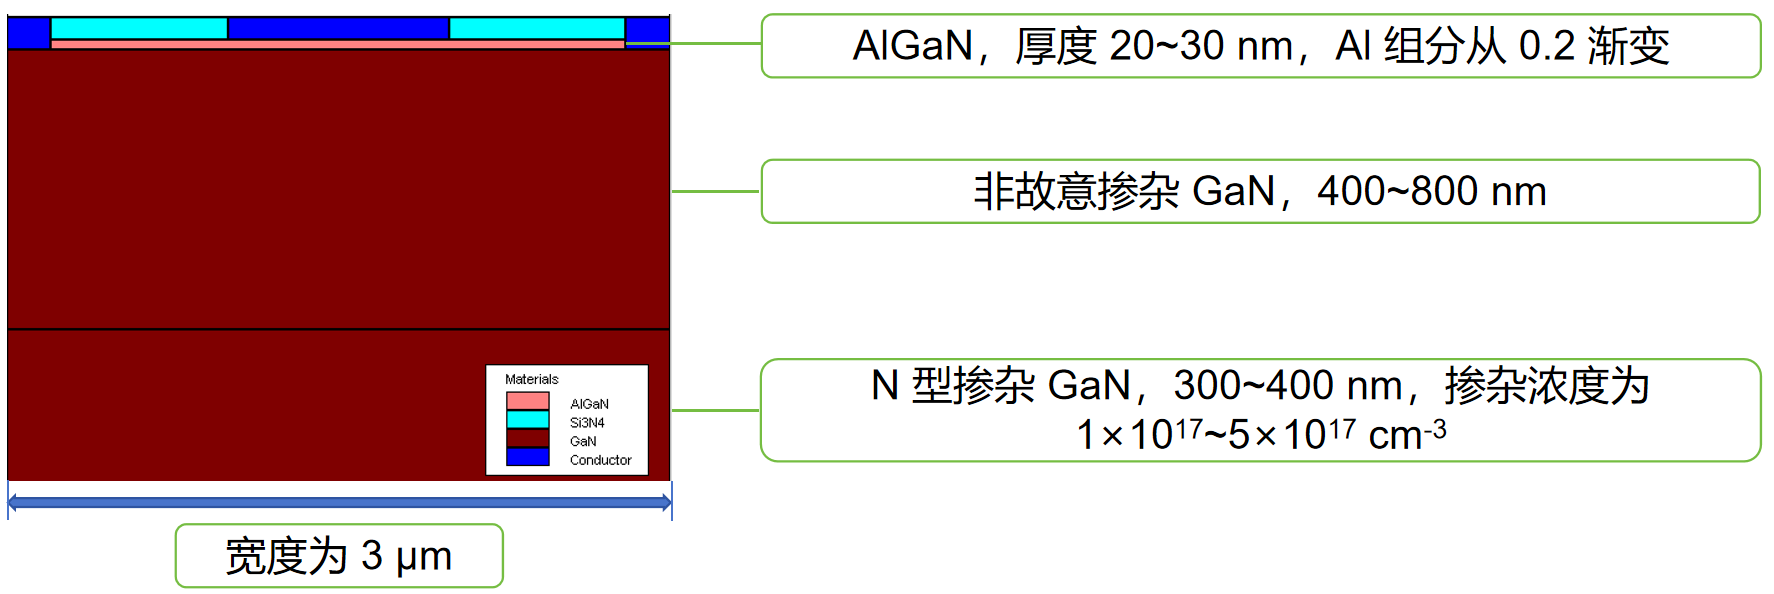
\includegraphics[width=\linewidth]{图片4.1.png}
	\caption{HEMT器件结构仿真参数设置}
\end{figure}

由于在实际情况下非故意掺杂生长的GaN通常带有非常强的背景掺杂浓度（约10\textsuperscript{15}\textasciitilde10\textsuperscript{17}cm\textsuperscript{-3}），这些非故意掺杂来自于生长系统中的SiO\textsubscript{2}杂质，以及GaN本身的晶体缺陷如氮空位等\cite{1021852996.nh}。而在仿真器中为绝对理想状态，不掺杂的GaN中的电子和空穴载流子则为绝对的平衡态，因此在仿真器中将非故意掺杂GaN层的掺杂浓度设置为10\textsuperscript{16}cm\textsuperscript{-3}，以模拟器件的现实情况。

在ICP工艺中，较难精确控制刻蚀深度，在对AlGaN进行刻蚀时可能会较难精确控制AlGaN层厚度，因此在仿真研究中本文将讨论AlGaN层厚度对器件性能的影响。

此外，我们在研究过程中发现，N型掺杂的GaN层的掺杂浓度和非故意掺杂的GaN层厚度会对器件性能造成较大影响。在本章中将对这些参数对比研究，以得出最佳的参数设置。

\subsection{转移特性与输出特性分析}

在第三章中提到，HEMT和MOSFET器件在同一外延层上且具有相同的层级架构，这是为了简化制备流程而做出的设计，在MOSFET器件中AlGaN层的厚度为150\,nm，并且Al组分由下至上从0.2线性渐变至0，在HEMT器件中需要将这一层刻蚀至20\textasciitilde30\,nm，因此HEMT中的AlGaN层的Al组分并不是理想状态下的均匀分布，而是从底部0.2开始渐变，经过换算可以得出其顶部Al组分应为0.173（20\,nm厚）、0.167（25\,nm厚）、0.16（30\,nm厚）。因此在对比研究AlGaN厚度变化的影响时应该同步改变仿真器中关于Al组分的设置。

\begin{figure}[H]
	\centering
	\begin{minipage}{0.48\linewidth}
		\centering
		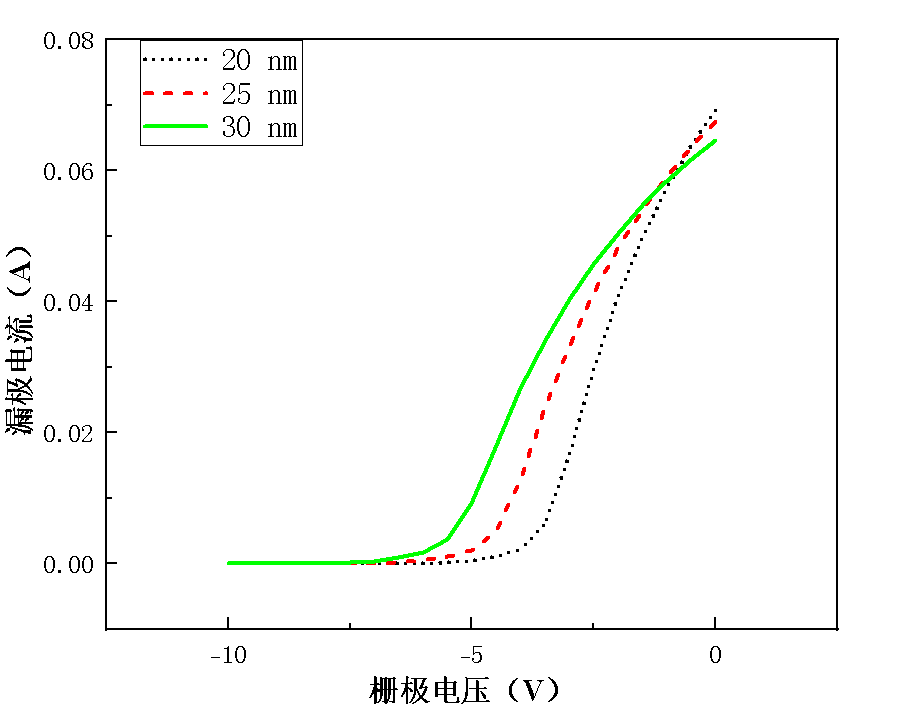
\includegraphics[width=\linewidth]{图片4.2.png}
		\caption{HEMT器件的转移特性曲线}
        \label{HEMT器件的转移特性曲线}
	\end{minipage} \hfill
	\begin{minipage}{0.48\linewidth}
		\centering
		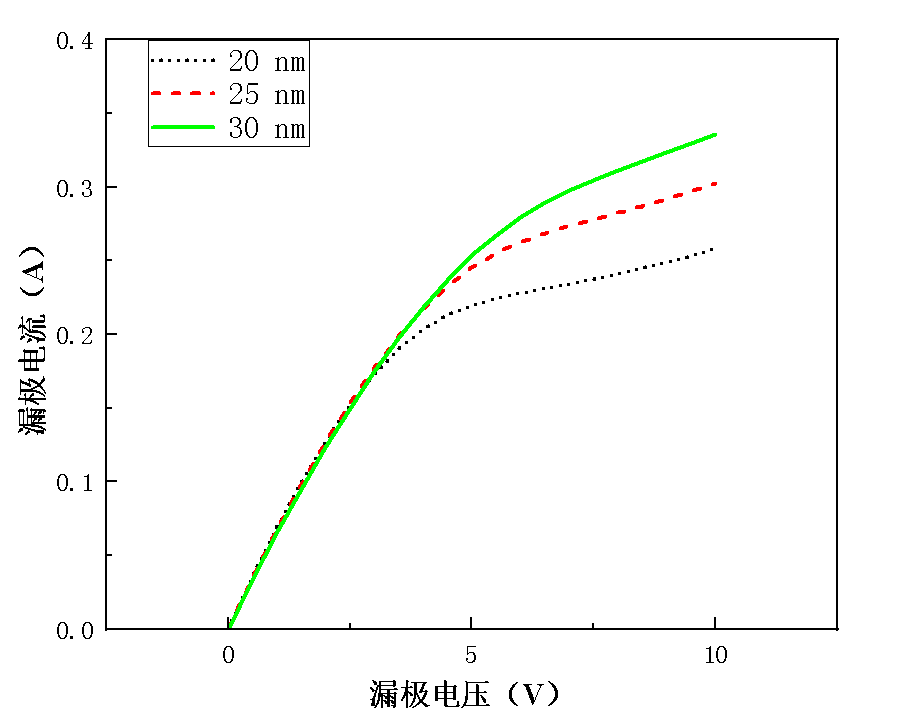
\includegraphics[width=\linewidth]{图片4.3.png}
		\caption{HEMT器件的输出特性曲线}
        \label{HEMT器件的输出特性曲线}
	\end{minipage}
\end{figure}

图\ref{HEMT器件的转移特性曲线}和图\ref{HEMT器件的输出特性曲线}分别为不同AlGaN层厚度下HEMT的转移特性曲线和输出特性曲线。其中测试转移特性时，漏极电压设置为1\,V，源极为0V，栅极从0\,V以-0.5\,V的幅度步退至-10\,V，从图中可见，随着AlGaN层厚度的增大，器件的关断电压也会减小，关断时的漏电流也会相应地增大，同时器件在开启状态时的电流也会有小幅度的减小；测试输出特性时栅压为0\,V，即器件处于完全开启状态，源极也同样为0\,V，漏极电压以0.5\,V为幅度步进至10\,V，由图可见AlGaN层厚度会影响饱和区的电流，导致饱和区电流减小。

对于出现这种现象的原因，可能是AlGaN层厚度增加，电子在沟道中传输时受到的散射几率会增大。这是因为较厚的AlGaN层会引入更多的杂质、缺陷等散射中心。根据conmob迁移率模型，杂质散射加剧会使载流子迁移率下降。同时栅极通过控制AlGaN/GaN异质结中势阱的深度来调节2DEG浓度，从而控制电流。当AlGaN层厚度增加时，栅极电压对势阱深度的调控能力会减弱。因为AlGaN层变厚，栅极电场穿透到异质结界面的难度增加，使得栅极电压对2DEG浓度的控制效果变差。

考虑到HEMT在电路中需要对电容进行快速充电，这要求其具有低导通电阻，也就是在特性曲线中显现出较高电流，因此20\,nm厚度的AlGaN层具有较好性能。此外，由于电极与AlGaN之间存在功函数差，在接触面会形成肖特基结，在栅极施加负压时会增大结深从而将2DEG中的电子耗尽，实现器件的关断，如果AlGaN的厚度过小（<20\,nm），0\,V栅极偏置下的结深就已经影响到了2DEG的形成。因此综合来看，20\,nm的厚度是最佳选择。但考虑到实际制备过程中的问题，可以在制备时适当加厚AlGaN层，尽量避免0\,V偏置时肖特基结对2DEG产生影响。

在研究不同参数对于器件性能影响过程中，通过转移特性曲线和输出特性曲线发现改变如器件宽度、衬底N型掺杂GaN厚度等参数时对曲线的影响并不明显，但在改变衬底掺杂浓度和非故意掺杂GaN层厚度时，曲线中会出现明显变化，如图\ref{不同掺杂浓度对HEMT转移特性和输出特性的影响}和图\ref{不同厚度对HEMT转移特性和输出特性的影响}所示：

\begin{figure}[H]
	\centering
	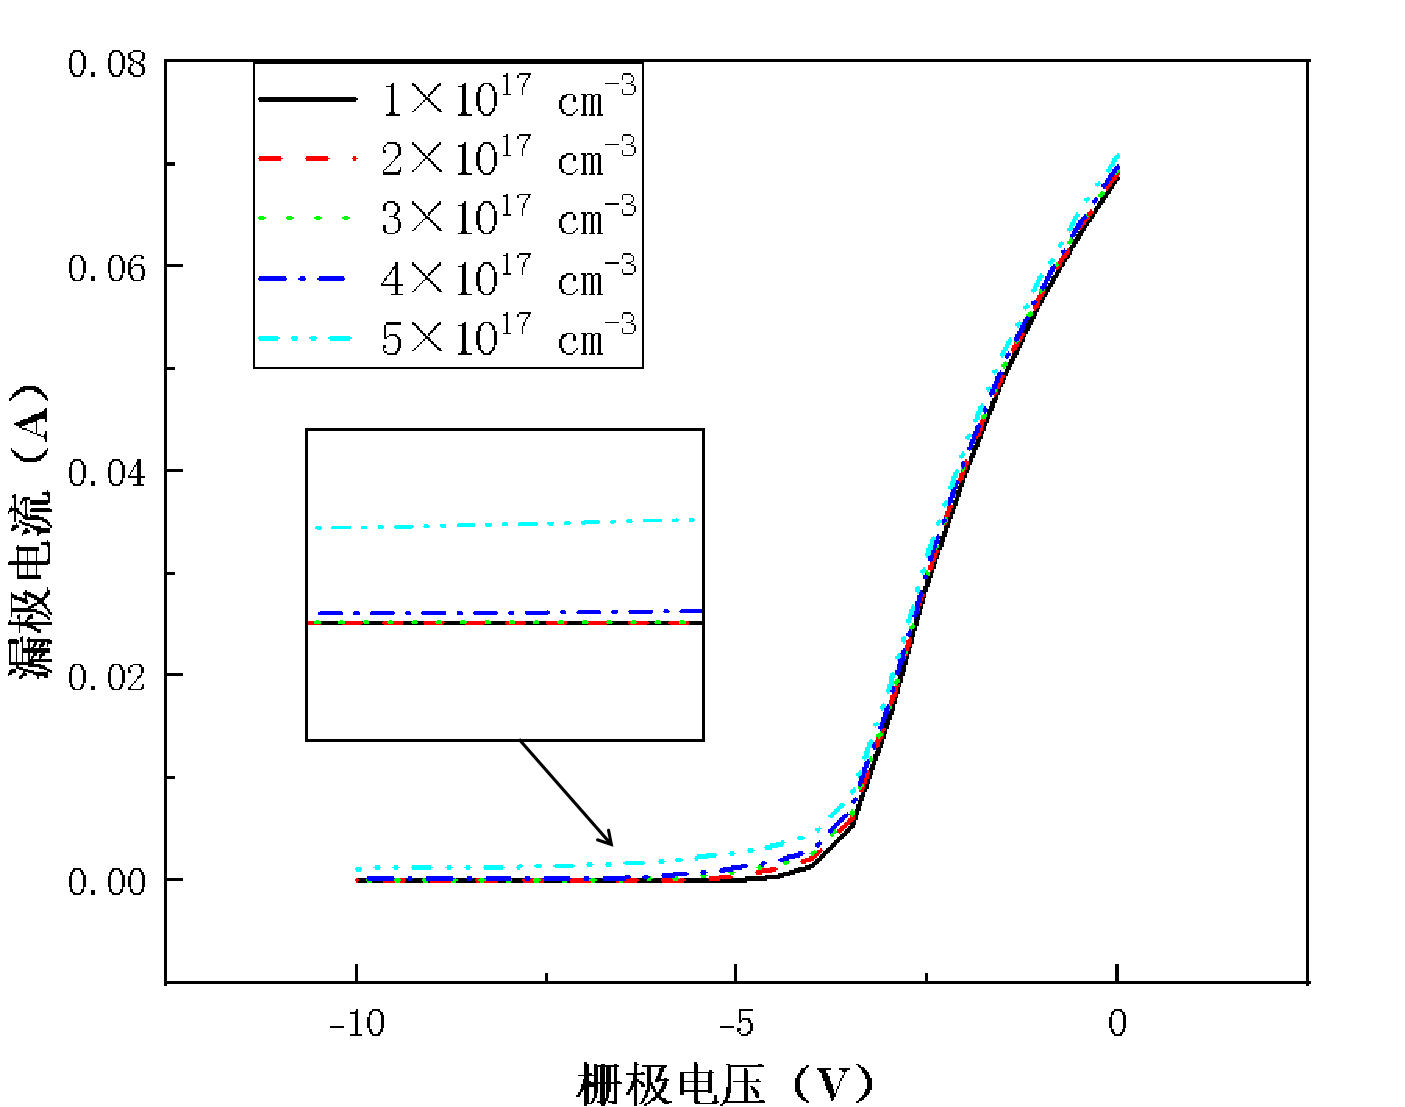
\includegraphics[width=0.48\linewidth]{图片4.41.png} \hfill
	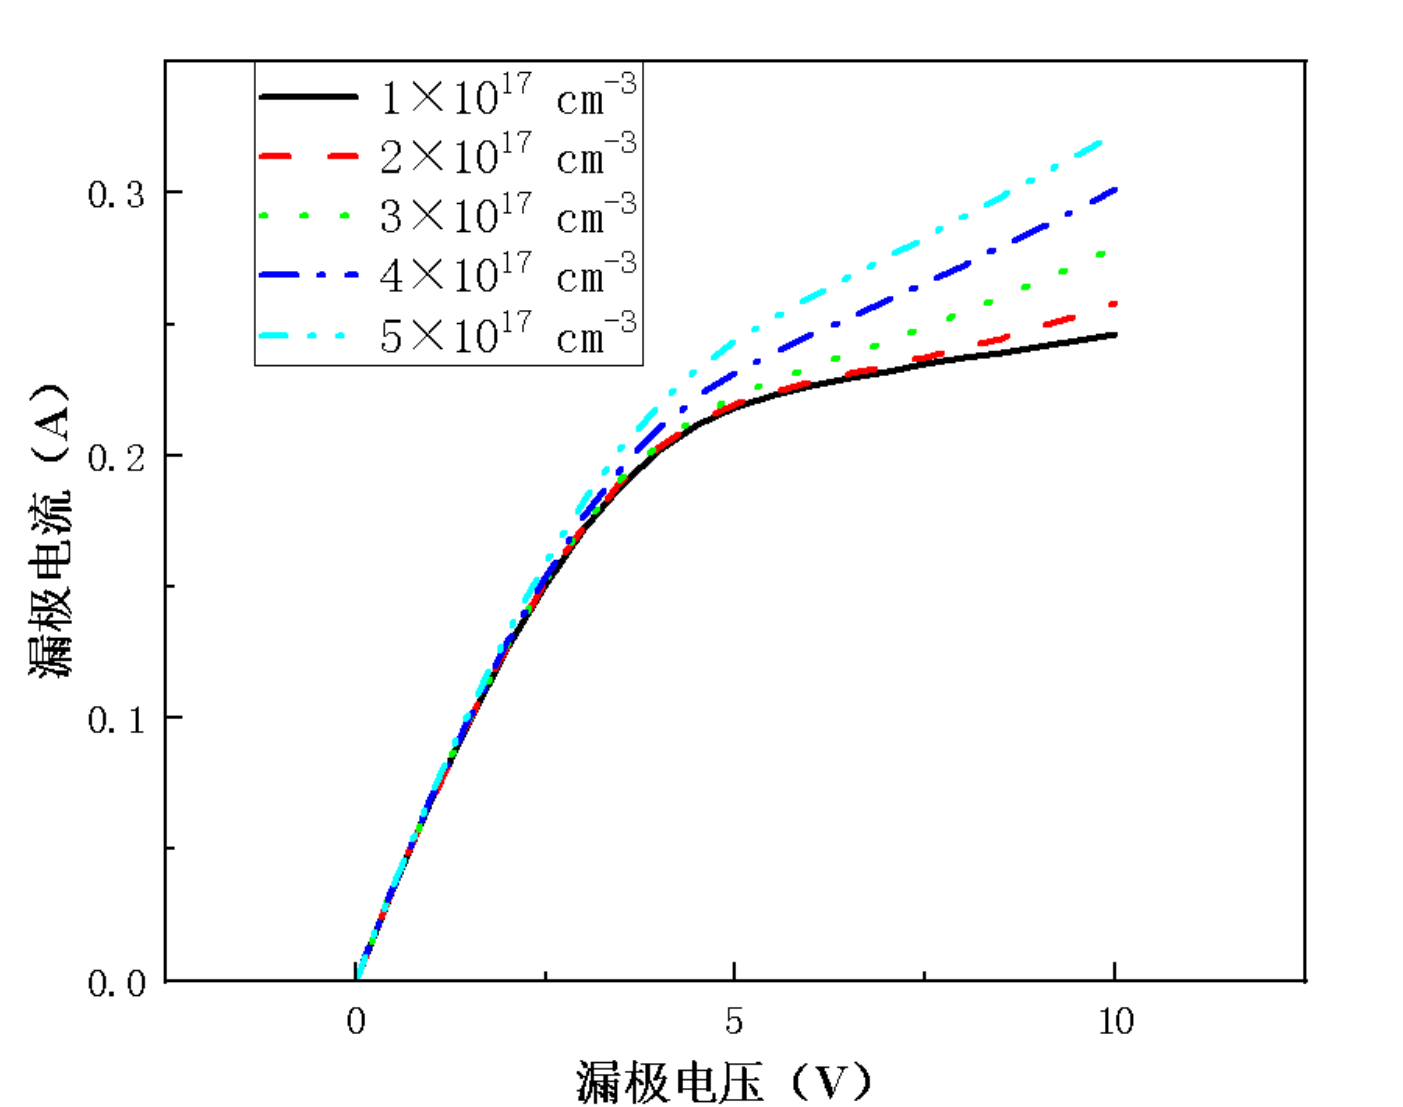
\includegraphics[width=0.48\linewidth]{图片4.42.png}
	\caption{不同掺杂浓度对HEMT转移特性和输出特性的影响}
    \label{不同掺杂浓度对HEMT转移特性和输出特性的影响}
\end{figure}

\begin{figure}[H]
	\centering
	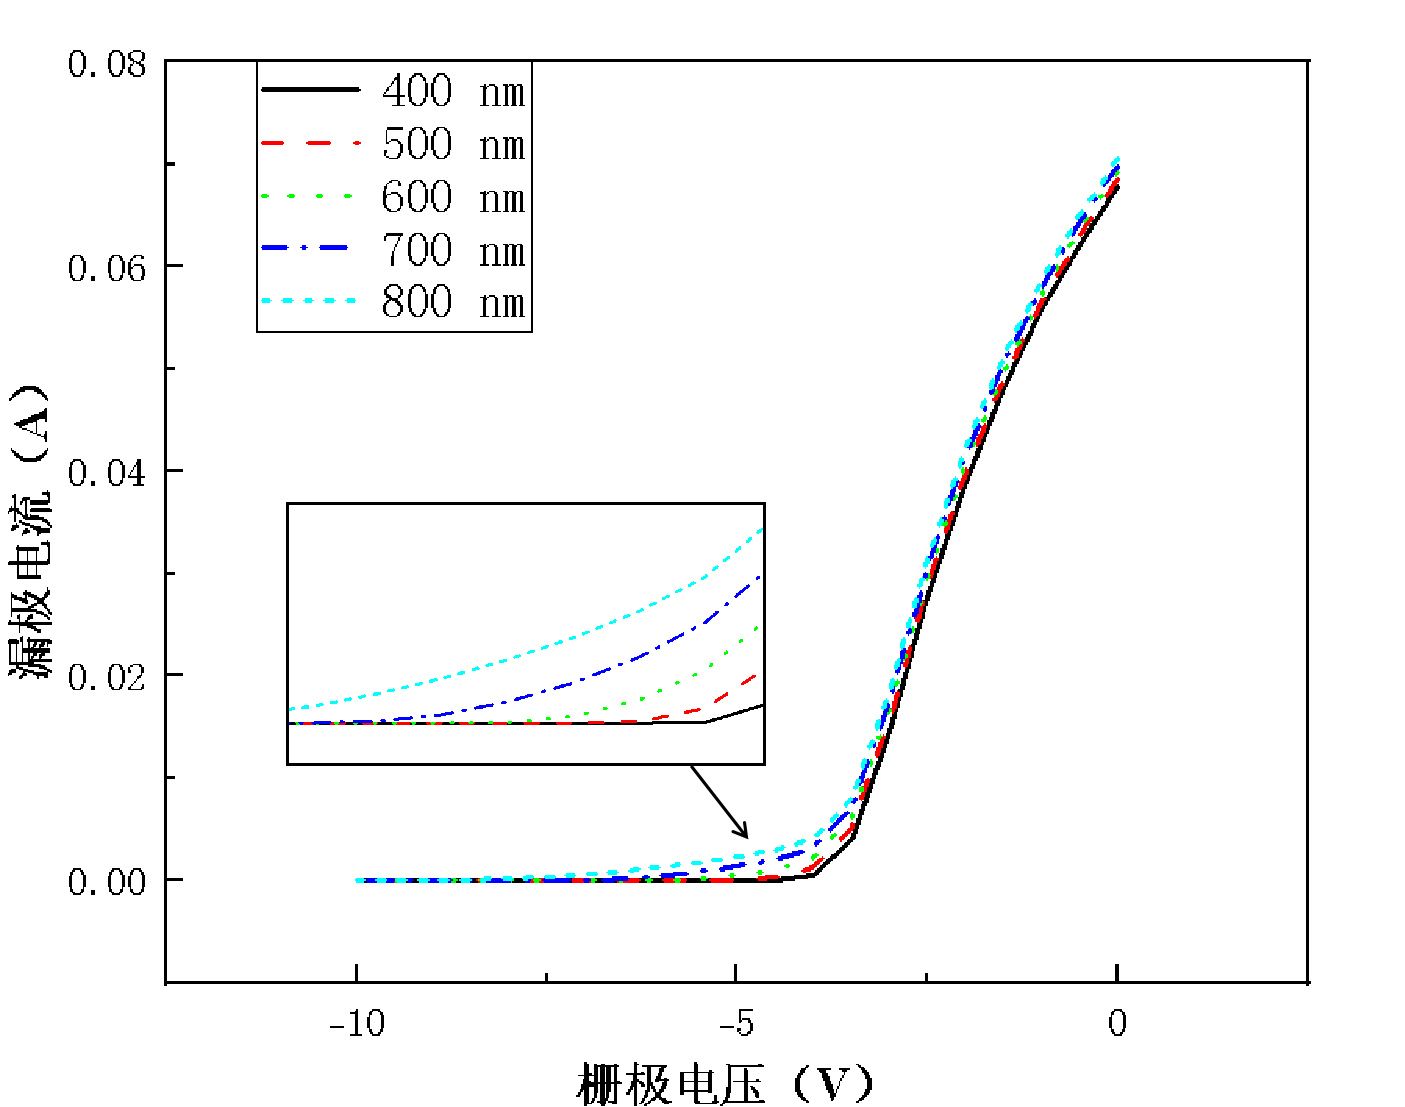
\includegraphics[width=0.48\linewidth]{图片4.51.png} \hfill
	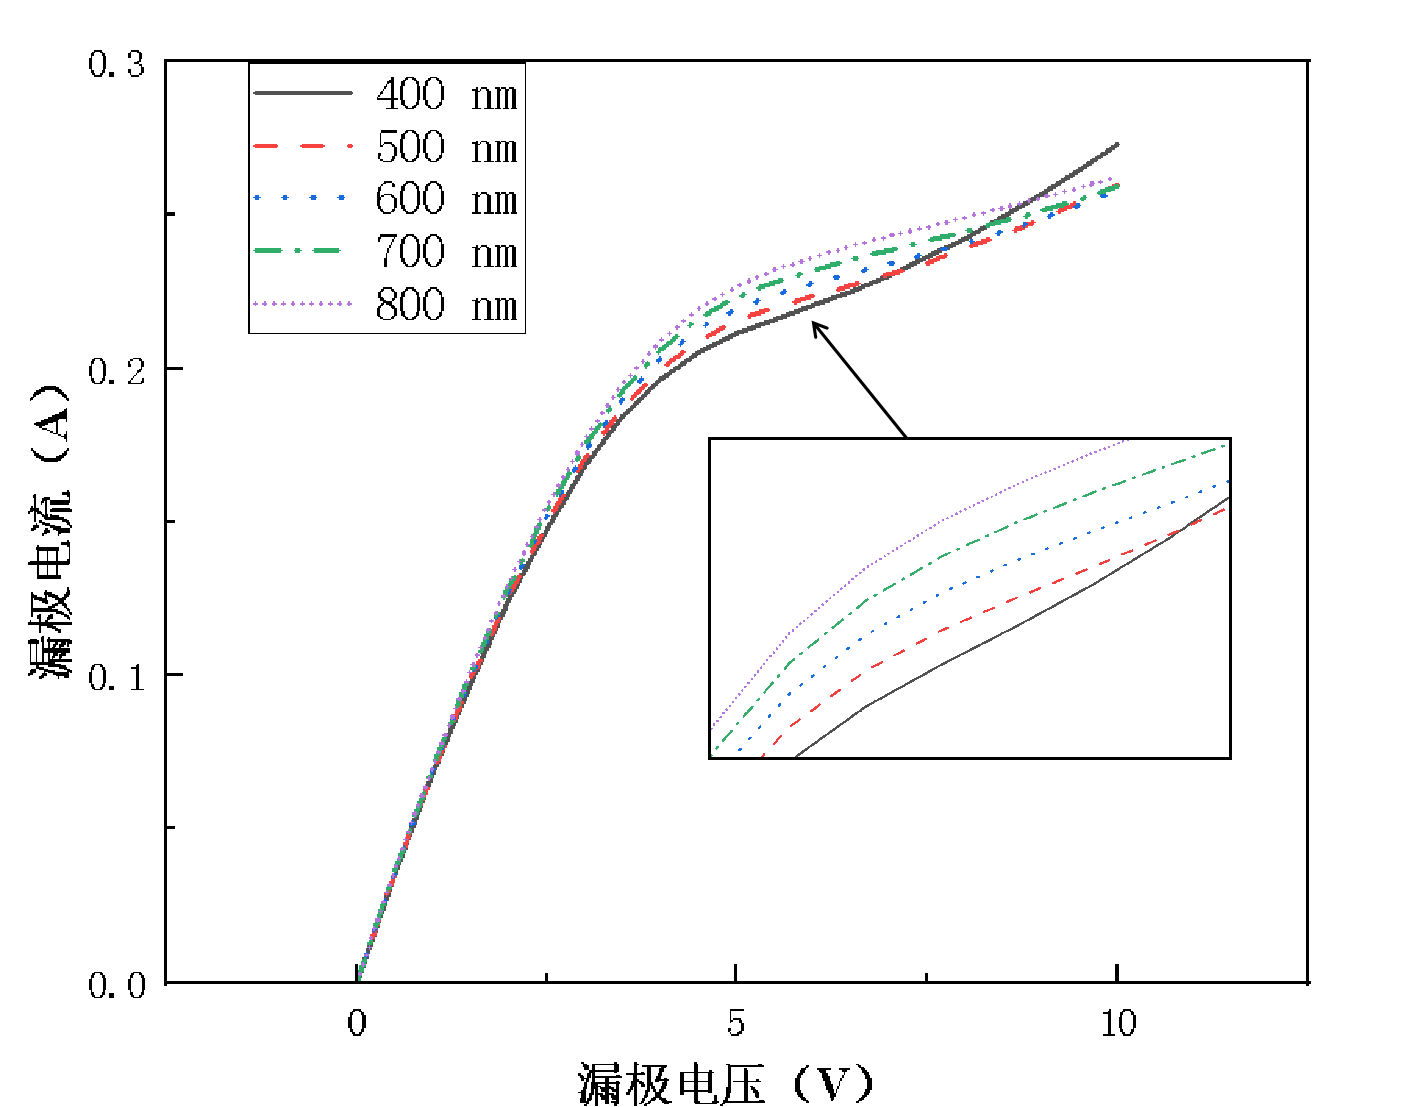
\includegraphics[width=0.48\linewidth]{图片4.52.png}
	\caption{不同厚度对HEMT转移特性和输出特性的影响}
    \label{不同厚度对HEMT转移特性和输出特性的影响}
\end{figure}

改变衬底掺杂浓度会导致漏极电压的增大，在转移曲线中栅极电压电压为0\,V时虽然变化不大，但在关断电压（约7.5\,V）时，会出现“夹不断”的现象，尤其在掺杂浓度为5×10\textsuperscript{17}cm\textsuperscript{-3}时关态漏电流已经非常明显。而在掺杂浓度增大的过程中关态漏电流也随之变大，在掺杂浓度为3×10\textsuperscript{17}cm\textsuperscript{-3}及以下时漏电流的大小小于10\textsuperscript{-5}量级，可认为是完全截断。这可能是由于衬底的重掺区和非故意掺杂区之间也会存在一个结，当栅极反偏想要耗尽2DEG中的电子时，这个结处于正向导通状态，下方重掺区的电子源源不断地进入上方，导致栅极的肖特基结不能完全耗尽电子，这一猜测将在下一小节载流子浓度分析时得到验证。

这一现象会导致在双晶体管集成器件在工作时的功耗增加，对器件的影响非常不利，因此在此方面考虑掺杂浓度应当尽量低。

但在输出曲线中，增加掺杂浓度显然会提升电流，高输出电流又是本器件地有效性能之一。因此，在权衡利弊之后，我们认为2×10\textsuperscript{17}cm\textsuperscript{-3}是一个比较好的掺杂浓度。

增加非故意掺杂层厚度时，转移曲线图中栅极关断电压显示出了“左移”的现象，也就是需要更低的电压才能将器件关断。出现此现象的原因应与上文提到的“耗不尽”现象同理，随着厚度增大，电子也会随之变多，也就需要更低的电压将电子完全耗尽。这就需要层厚尽量低以提升栅控能力。

随着非故意掺杂层厚度增加，输出曲线中的漏电流整体略微减小，但在最后漏电压为10\,V时，出现了先减小（从400\,nm到600\,nm）后增大（从600\,nm到800\,nm）的趋势。对于出现这一现象的原因我们尚未探究清楚，希望通过后续的研究可以找出原因。

本节通过对电学特性曲线地分析，得出了器件较为合适的参数设置值，并对某些现象做出了猜测，在下一小节中将对这些猜测进行分析验证。

\subsection{载流子浓度与能带分析}

HEMT在所有电极均为零偏置时处于导通状态，在GaN和AlGaN接触面形成二维电子气（2DEG），如图\ref{HEMT开启状态的电子浓度示意图}所示：

\begin{figure}[H]
	\centering
	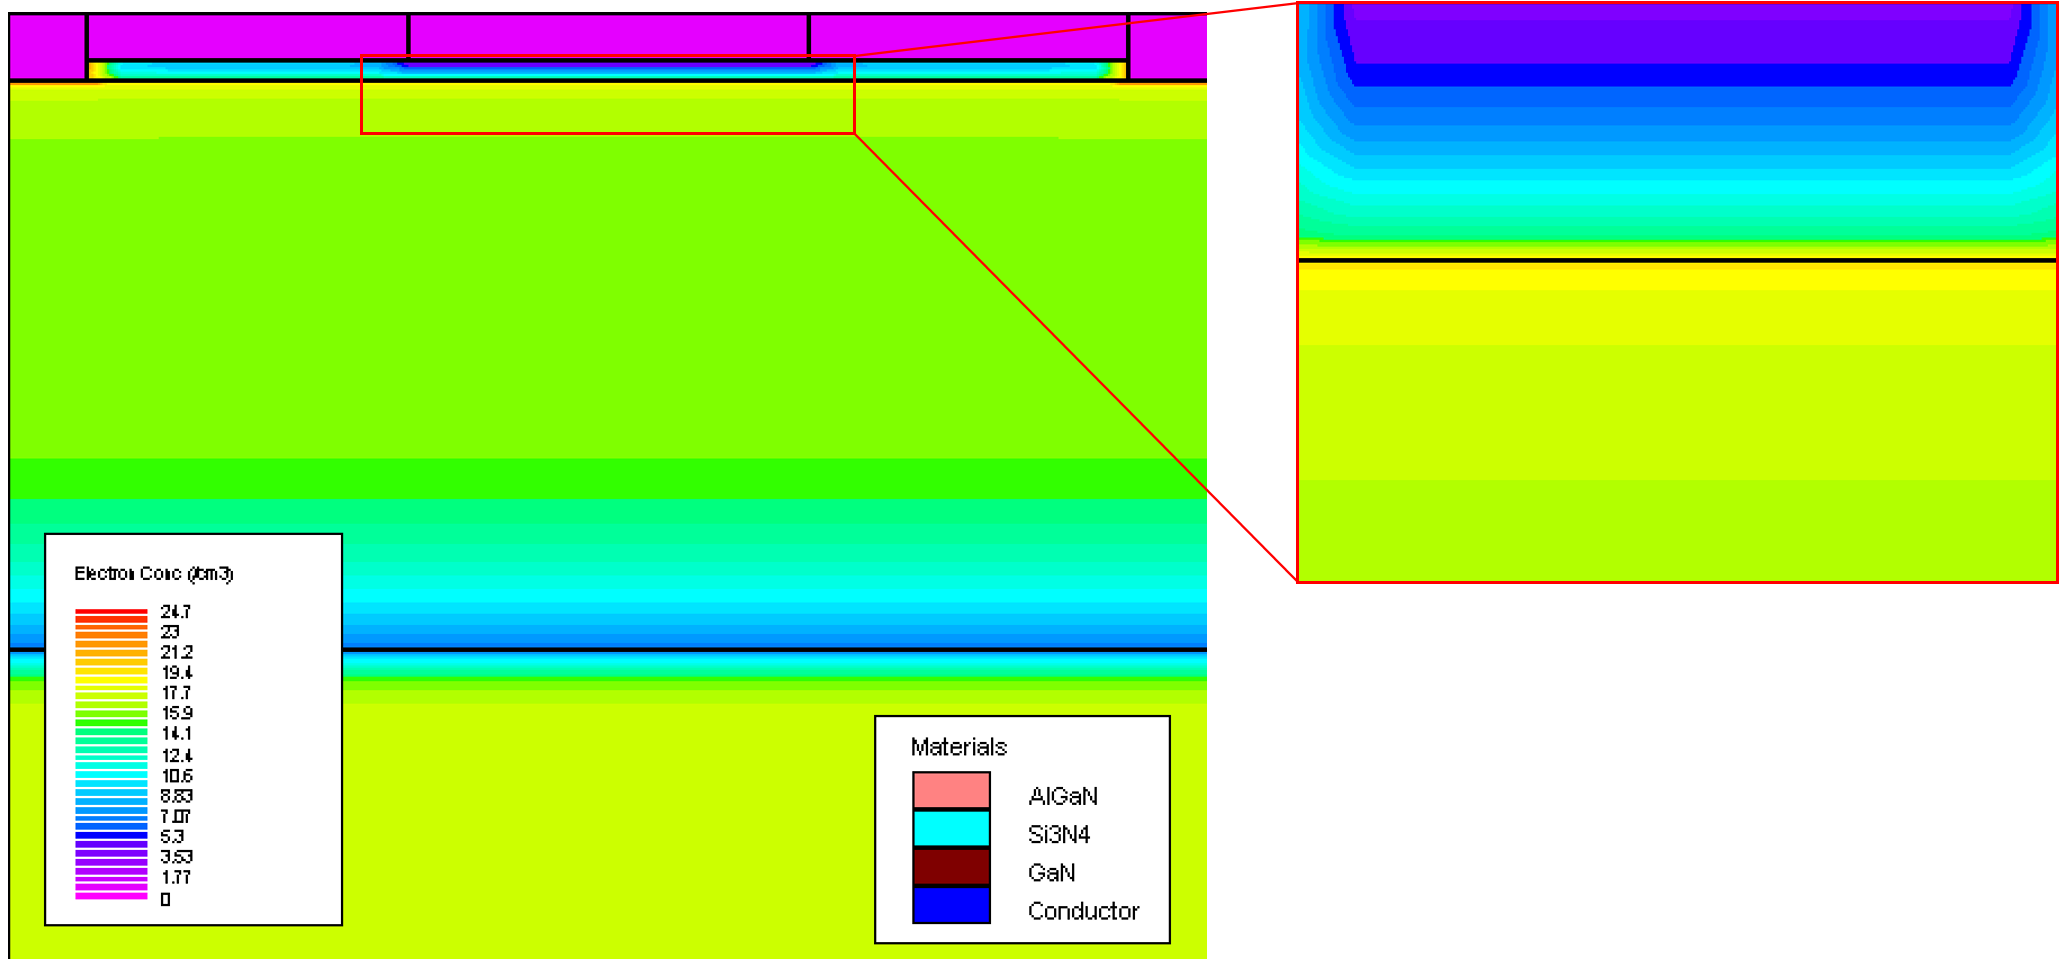
\includegraphics[width=0.75\linewidth]{图片4.6.png}
	\caption{HEMT开启状态的电子浓度示意图}
    \label{HEMT开启状态的电子浓度示意图}
\end{figure}

由图中可见，在2DEG区域电子浓度升高至10\textsuperscript{20}cm\textsuperscript{-3}，高电子浓度保证了器件的输出性能。但在图中不难发现，非故意掺杂GaN层和衬底N型掺杂GaN层之前形成了耗尽区，也就是一个N\textsuperscript{+}与N\textsuperscript{-}型的结，在其中存在反向电场阻止重掺区的电子向上扩散，但当栅极施加负电压时，会抵消反向电场的作用，使耗尽区减小，下方的电子源源不断地进入上方区域。

\begin{figure}[H]
	\centering
	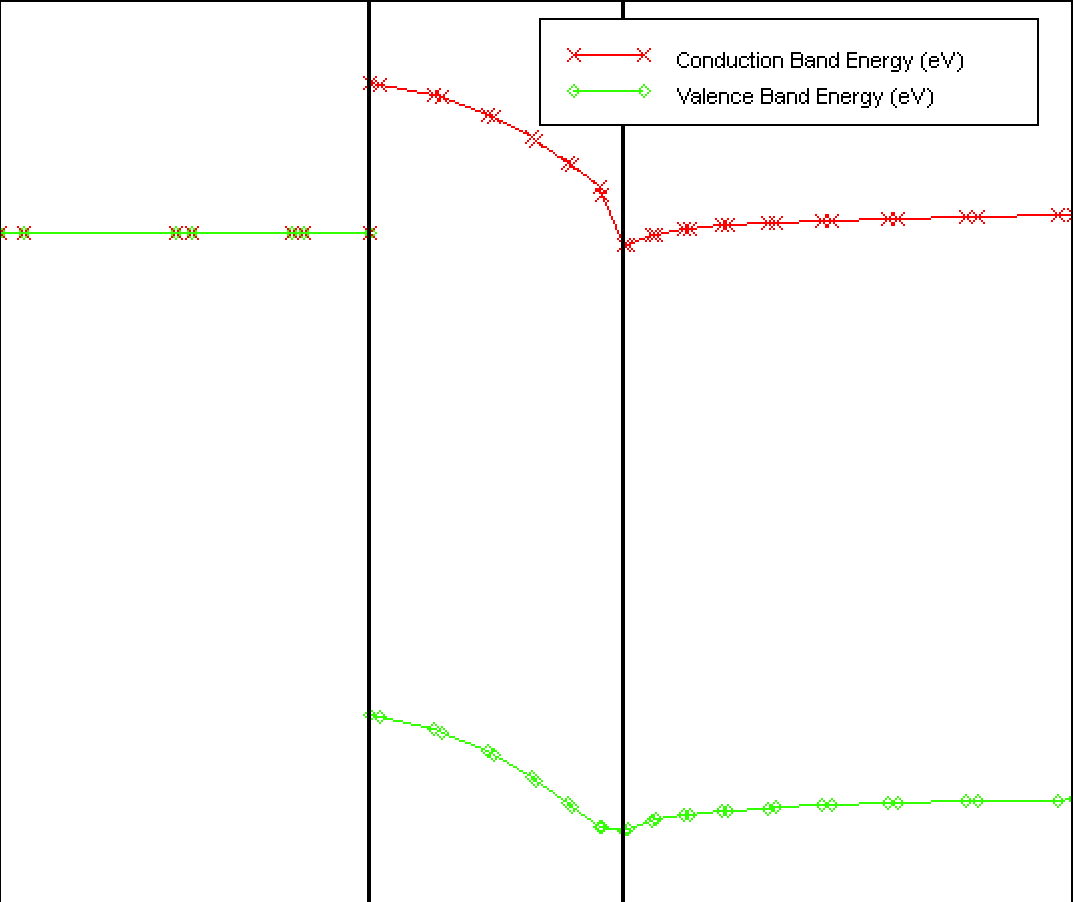
\includegraphics[width=0.5\linewidth]{图片4.7.png}
	\caption{HEMT的能带图}
    \label{HEMT的能带图}
\end{figure}

图\ref{HEMT的能带图}是通过使用Tonyplot地cutline功能显示出来的能带图，左侧为栅电极，中部为AlGaN，右侧则为非故意掺杂的GaN。从能带图也可以看出，器件处于导通状态时，在AlGaN和GaN界面处会形成电子肼，吸引电子聚集在交界处，形成2DEG。

当器件处于关断状态时，栅电极和AlGaN之间形成的肖特基结耗尽区会扩大至非故意掺杂GaN层内，将电子全部耗尽，如图\ref{关断状态的HEMT电子浓度图}所示。

\begin{figure}[H]
	\centering
	\begin{minipage}{0.48\linewidth}
		\centering
		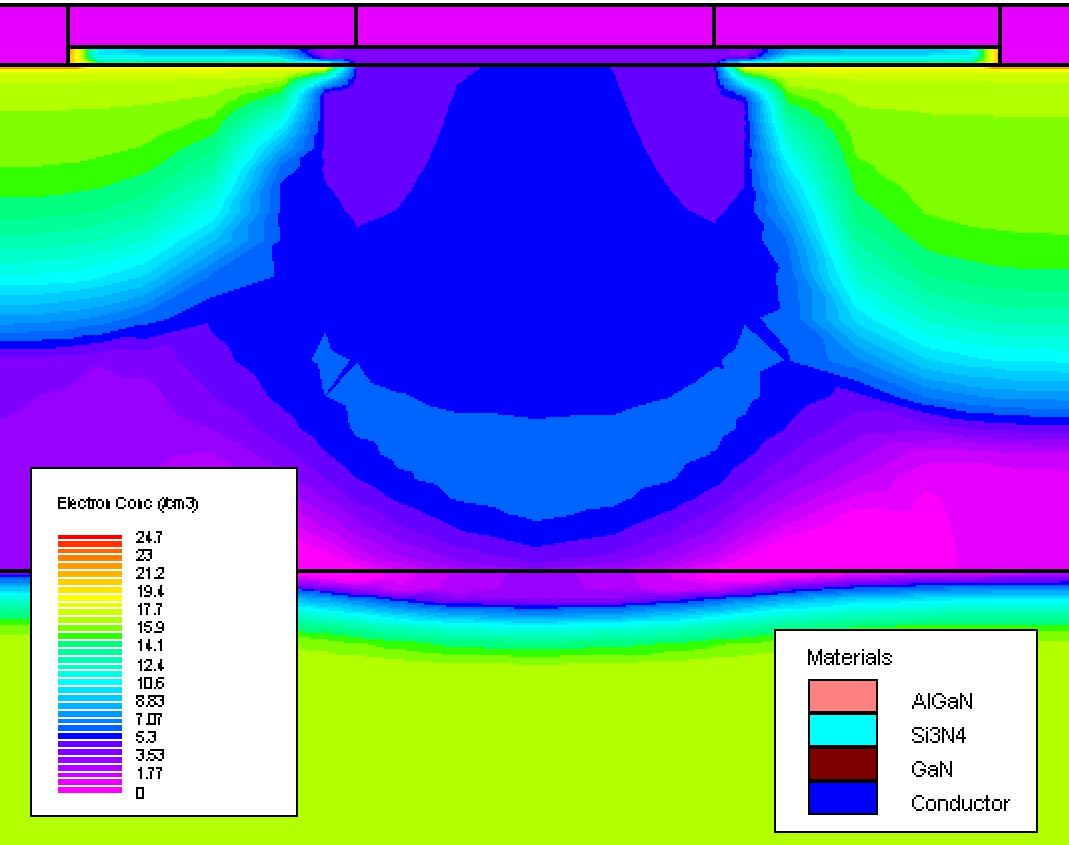
\includegraphics[width=\linewidth]{图片4.8.png}
		\caption{关断状态的HEMT电子浓度图}
        \label{关断状态的HEMT电子浓度图}
	\end{minipage} \hfill
	\begin{minipage}{0.48\linewidth}
		\centering
		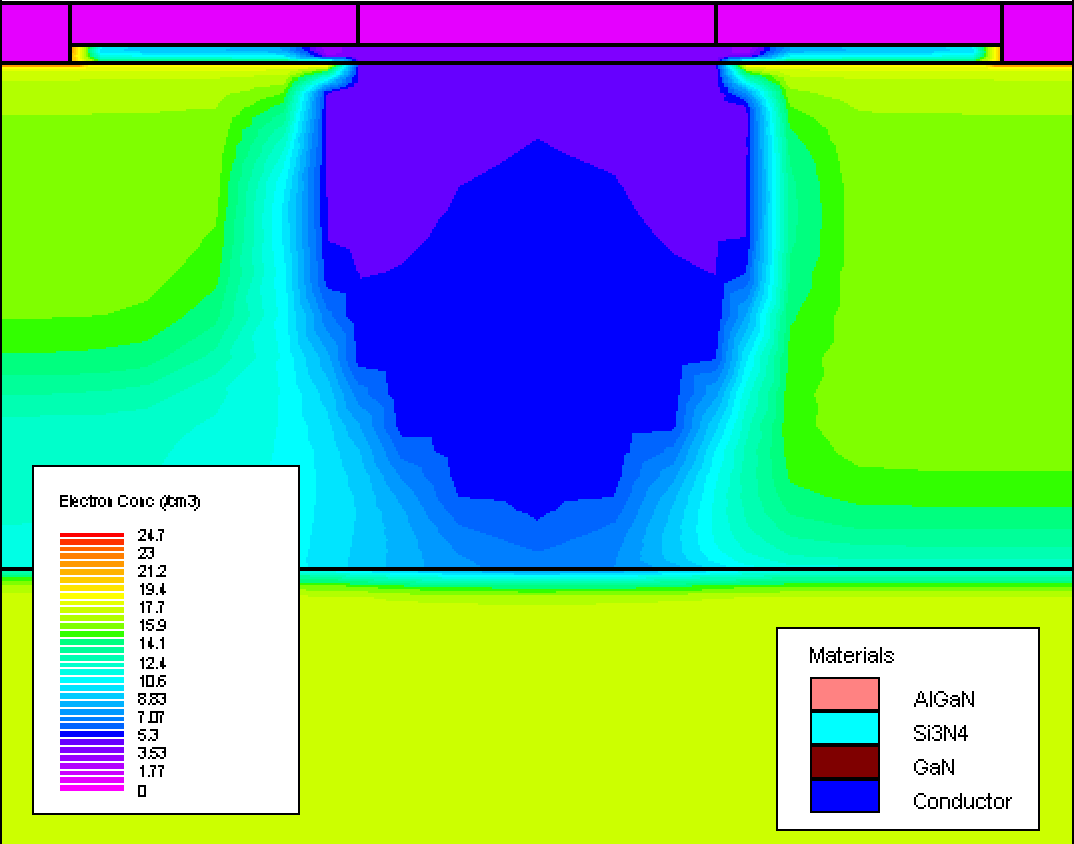
\includegraphics[width=\linewidth]{图片4.9.png}
		\caption{掺杂浓度提升后的HEMT}
        \label{掺杂浓度提升后的HEMT}
	\end{minipage}
\end{figure}

如果将衬底重掺区掺杂浓度提升，则会出现“耗不尽”的现象，如图\ref{掺杂浓度提升后的HEMT}所示。由于栅电极和AlGaN之间形成的肖特基结不能将非故意掺杂区中的电子完全耗尽，会导致非故意掺杂区和衬底重掺区之间形成电流通路，电子可以通过这条通路从源极抵达栅极，造成漏电流问题。解决此问题的方法为减小重掺区掺杂浓度，但减小浓度又会对器件开启时的饱和电流有所影响，因此需要均衡考虑两方面因素，选择最佳的掺杂浓度参数设置。仿真软件在这个过程中显得极其重要，在本文研究过程中通过调整各种数值最终找出了导致器件关态“耗不尽”的原因为衬底掺杂过高，然后通过调整参数设置找出最佳掺杂浓度为2×10\textsuperscript{17}cm\textsuperscript{-3}，如果没有仿真软件参与，实际器件制备则会浪费大量时间，甚至导致研究失败。

\section{MOSFET器件的特性分析}

MOSFET在GaN基驱动集成器件中作为驱动管，需将存储电容的电压信号稳定转换为驱动电流。因此要重点研究其栅极电压—漏极电流（V\textsubscript{gs}-I\textsubscript{ds}）线性度以及饱和区恒流特性，确保Micro-LED亮度与数据电压精准匹配。

本文在上一节中研究并讨论了HEMT的结构参数设置，而MOSFET和HEMT具有相同层级架构。在仿真研究过程中发现，上节中结构参数的调整（衬底掺杂、非故意掺杂层厚度）对MOSFET的性能影响十分有限。由于HEMT的AlGaN是通过刻蚀达到预定厚度，存在刻蚀不精确的问题，因此需要讨论厚度对HEMT器件性能的影响，而在MOSFET中通过沉积形成的AlGaN则没有此问题，因此并不讨论。

在仿真器中MOSFET的剖面图及结构参数设置如图\ref{MOSFET的剖面图及结构参数}所示：

\begin{figure}[H]
	\centering
	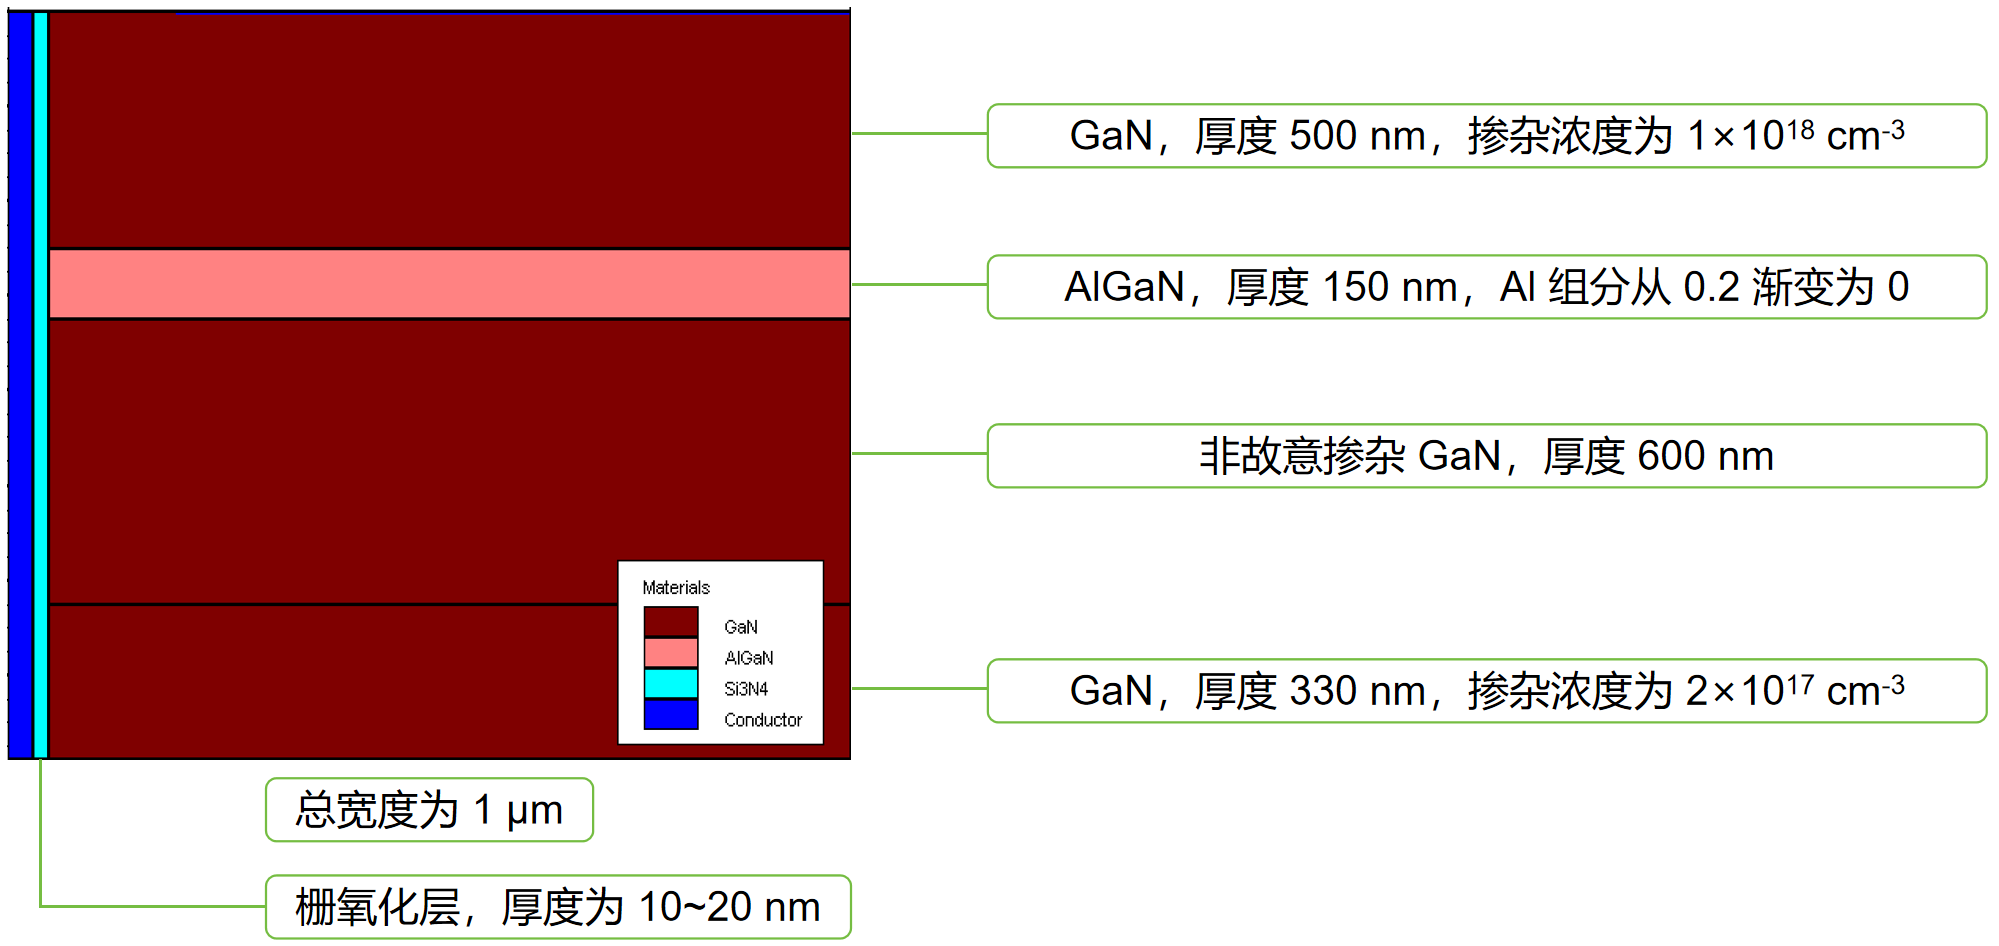
\includegraphics[width=\linewidth]{图片4.10.png}
	\caption{MOSFET的剖面图及结构参数}
    \label{MOSFET的剖面图及结构参数}
\end{figure}

各层级的厚度、掺杂等参数则使用了本章上节分析HEMT时获得的合适参数值，对于MOSFET最重要的栅氧化层厚度，将在本节讨论并分析。

\subsection{转移特性和输出特性分析}

MOSFET的性能指标，即栅极电压—漏极电流（V\textsubscript{gs}-I\textsubscript{ds}）线性度以及饱和区恒流特性，能够在转移曲线和输出曲线中得到很好的体现。这些特性与栅氧化层的厚度有着密切联系，下面将比较10\,nm、15\,nm、20\,nm的栅氧化层厚度下，MOSFET的性能指标变化。

\begin{figure}[H]
	\centering
	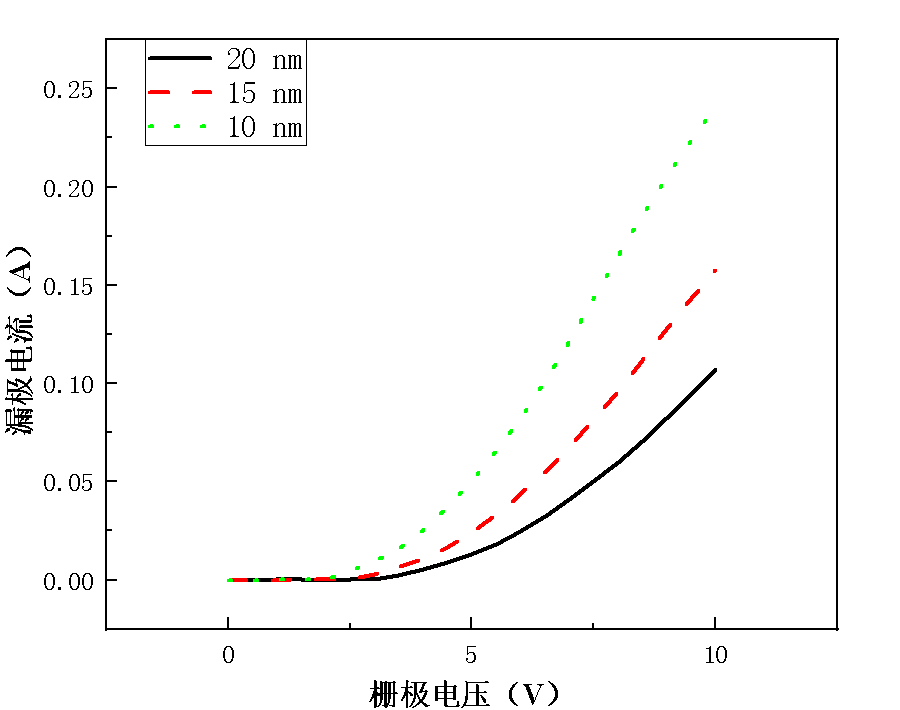
\includegraphics[width=0.48\linewidth]{图片4.111.png} \hfill
	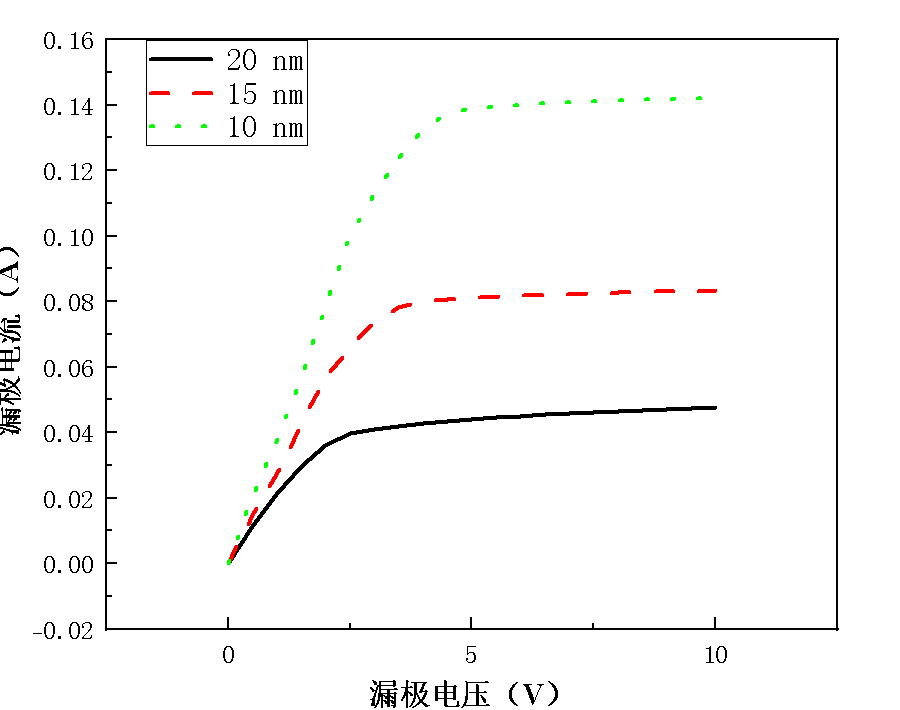
\includegraphics[width=0.48\linewidth]{图片4.112.png}
	\caption{MOSFET的转移曲线（左）和输出曲线（右）}
    \label{MOSFET的转移曲线（左）和输出曲线（右）}
\end{figure}

图\ref{MOSFET的转移曲线（左）和输出曲线（右）}分别是MOSFET的转移曲线（左）和输出曲线（右）图。从转移曲线图中可见，栅氧化层减小后，MOSFET的开启电压会随之减小，在达到5\,V的工作电压后电压—漏极电流（V\textsubscript{gs}-I\textsubscript{ds}）也会更加符合线性的要求。从输出曲线图中可以发现，随着栅氧化层厚度的减小，其饱和电流在增大的同时，饱和区电流变化也会更小，同样符合性能指标的要求。但考虑到仿真器处于完全理想状态，在实际器件中栅氧化层厚度过小可能会引发栅极漏电流问题，使得电容在充放电过程中电压产生的变化过大。这不仅会导致器件工作状态功耗增加，还有可能引发器件工作状态进入放大区。可见栅氧化层厚度应当不宜过大，因此本文中采用15\,nm的厚度进行研究。

\subsection{载流子浓度与能带分析}

MOSFET在零栅压（V\textsubscript{gs}=0\,V）时，GaN表面呈高阻态，此时器件依赖AlGaN渐变层的极化效应形成高浓度空穴区。如图\ref{MOSFET中的空穴浓度（左）和电子浓度（右）}所示，AlGaN层从下至上Al组分从0.2线性降至0，形成三维空穴气（3DHG）层。

通过Tonyplot提取界面处载流子浓度分布可见，如图\ref{MOSFET中的空穴浓度（左）和电子浓度（右）}中所示，3DHG区域空穴浓度高达10\textsuperscript{18}cm\textsuperscript{-3}，显著高于传统Mg掺杂P型GaN（约5×10\textsuperscript{17}cm\textsuperscript{-3}），且分布更均匀（横向浓度波动更小）。这是由于极化效应直接通过晶格应变产生电荷累积，避免了Mg掺杂的激活效率低和高温退火缺陷。

\begin{figure}[H]
	\centering
	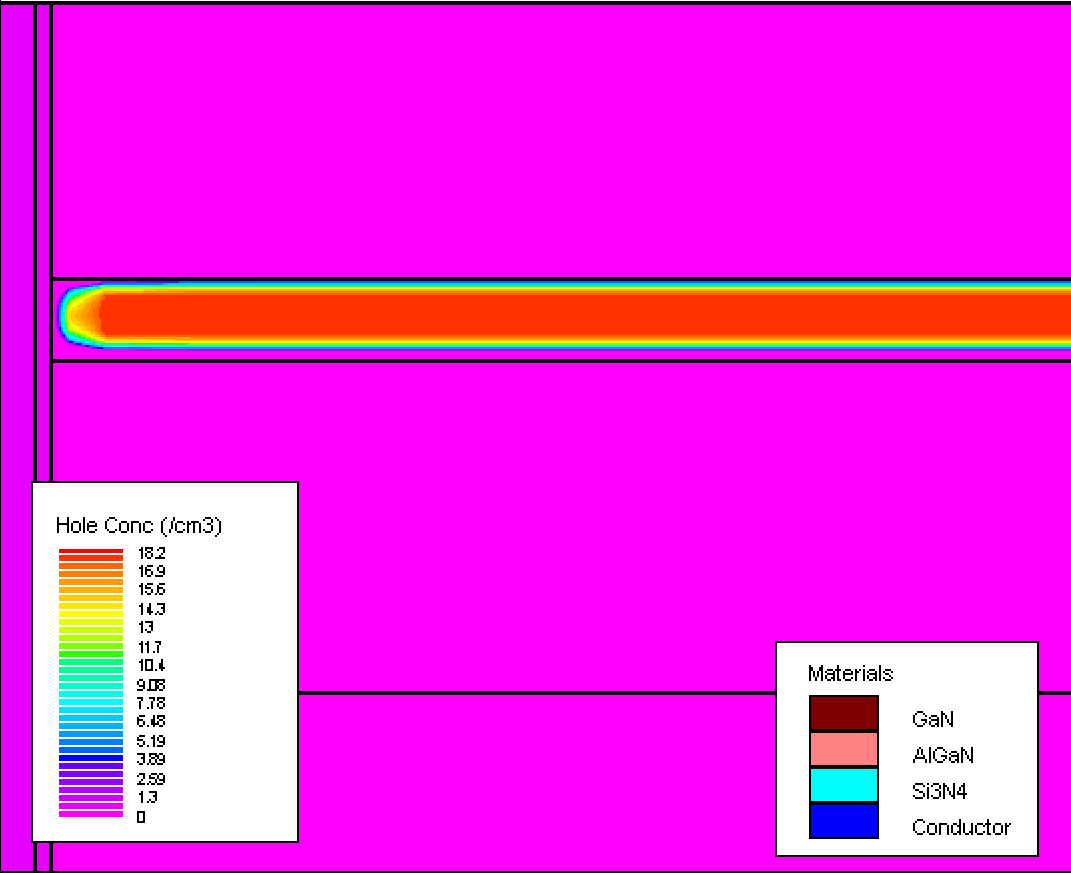
\includegraphics[width=0.48\linewidth]{图片4.121.png} \hfill
	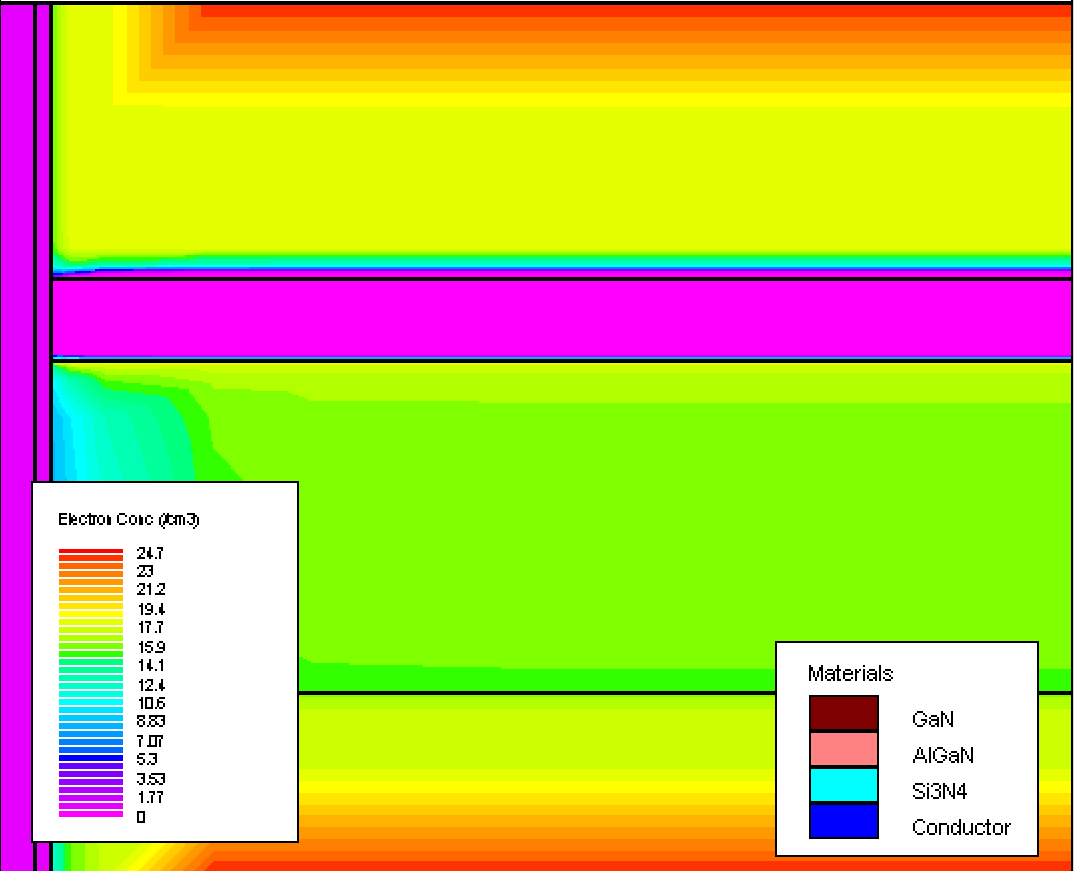
\includegraphics[width=0.48\linewidth]{图片4.122.png}
	\caption{MOSFET中的空穴浓度（左）和电子浓度（右）}
    \label{MOSFET中的空穴浓度（左）和电子浓度（右）}
\end{figure}

当栅极施加正电压（如V\textsubscript{gs}=7.5\,V），栅氧化层（Si\textsubscript{3}N\textsubscript{4}）右方的电场穿透至GaN表面，吸引电子在表面形成N型反型沟道，连接源极与漏极。如图\ref{MOSFET开启时的电子浓度}所示，在左侧反型沟道已形成，电子浓度达10\textsuperscript{18}cm\textsuperscript{-3}。

\begin{figure}[H]
	\centering
	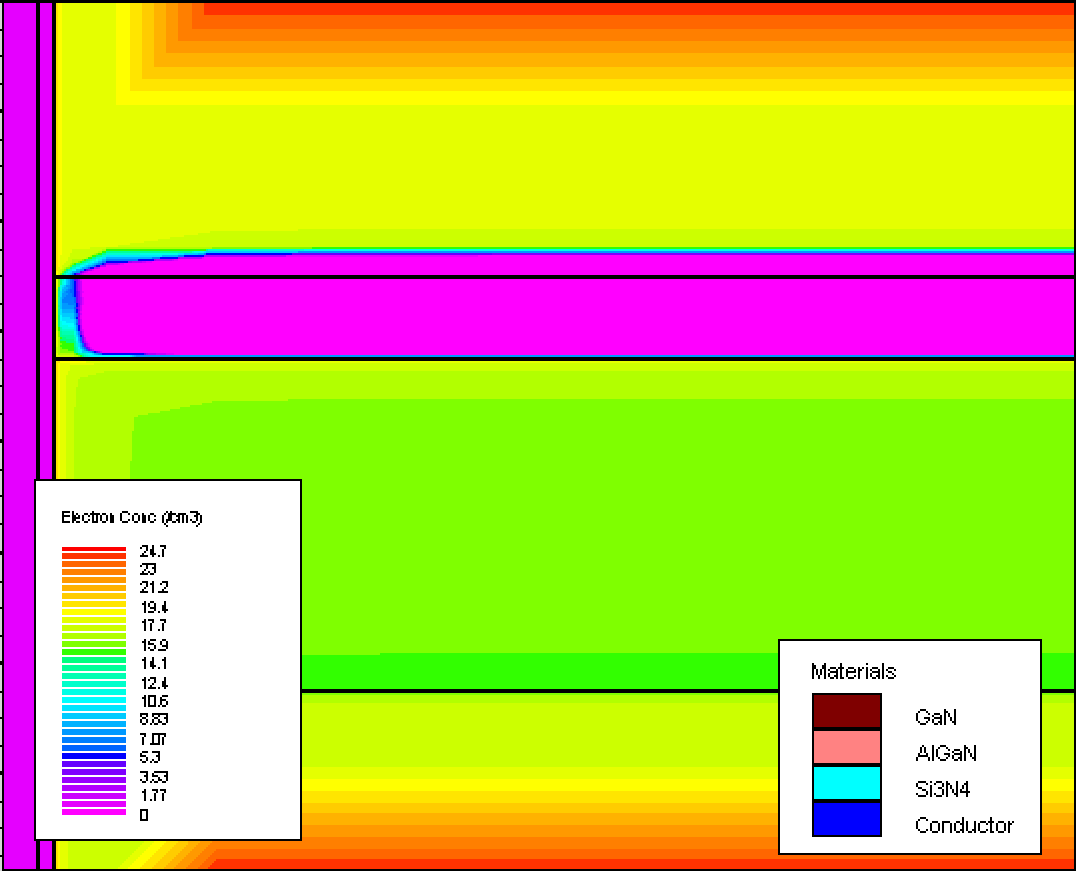
\includegraphics[width=0.5\linewidth]{图片4.13.png}
	\caption{MOSFET开启时的电子浓度}
    \label{MOSFET开启时的电子浓度}
\end{figure}

在器件分别处于关断和开启状态时，使用cutline工具观察栅氧化层下方的能带变化，如图\ref{MOSFET关断（左）和开启（右）时的能带图}所示：

\begin{figure}[H]
	\centering
	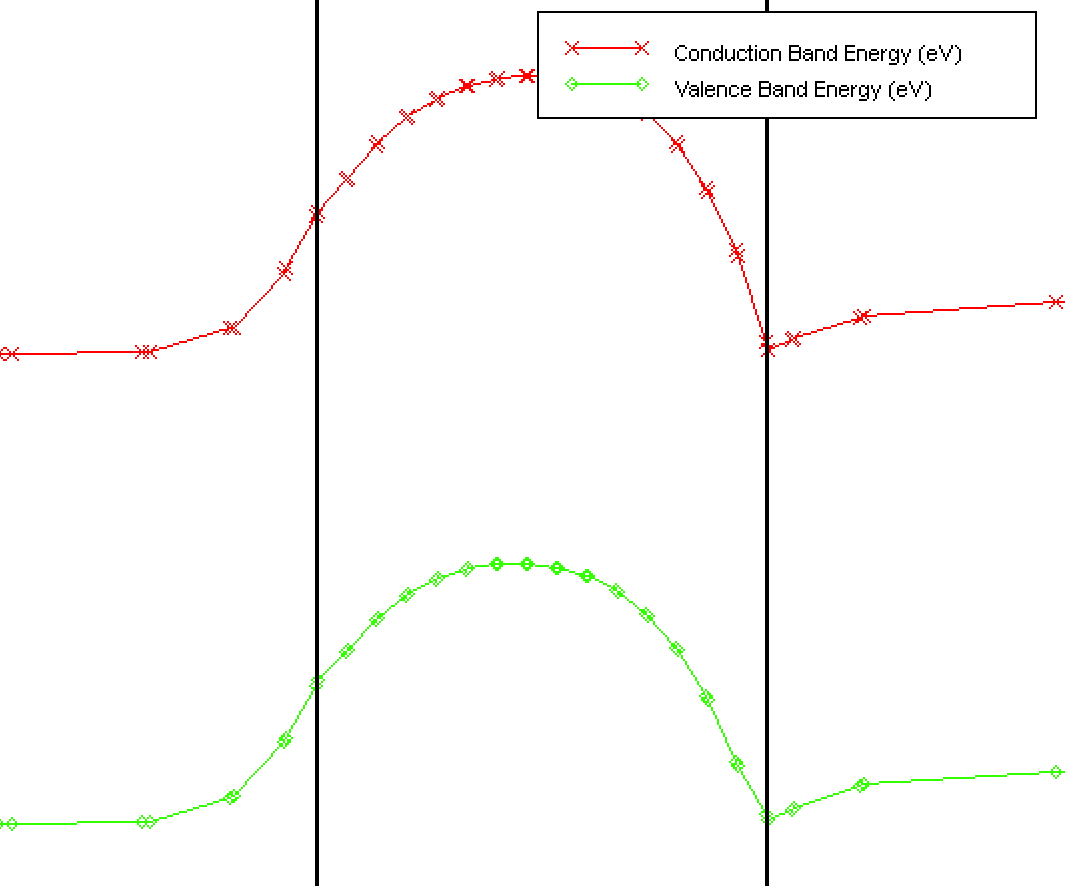
\includegraphics[width=0.48\linewidth]{图片4.141.png} \hfill
	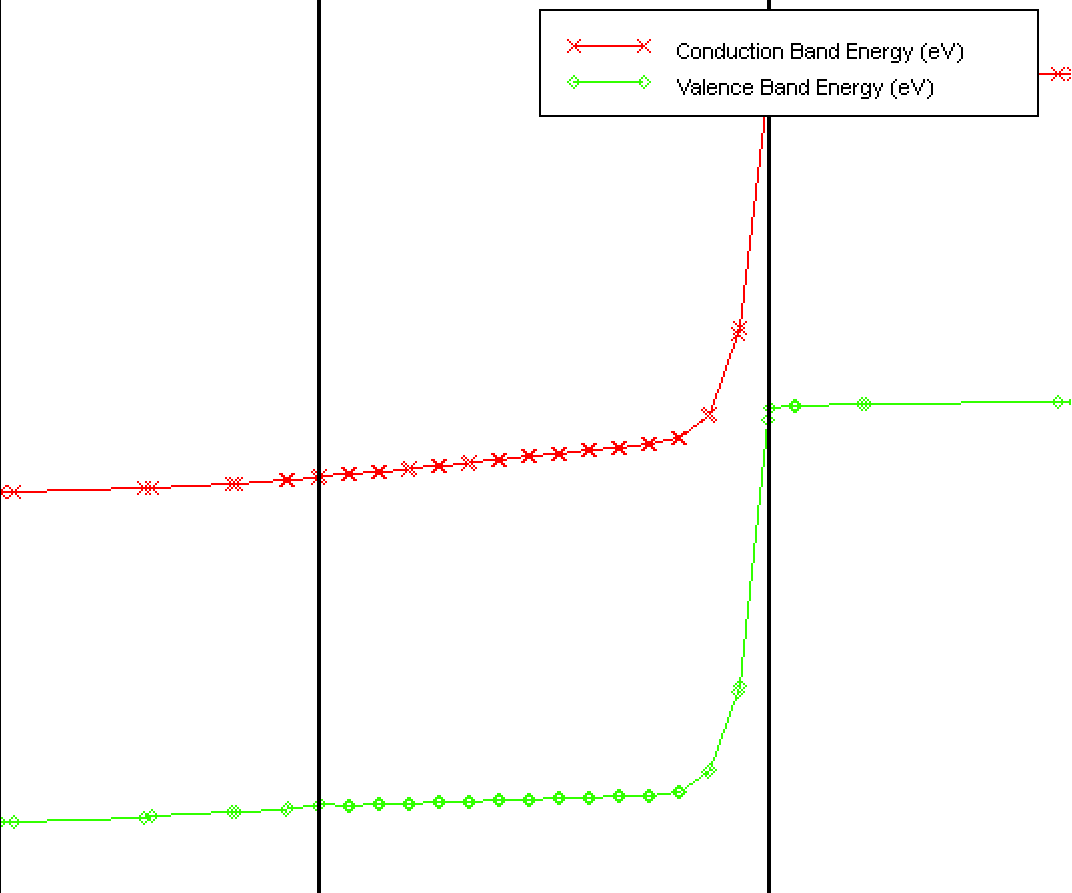
\includegraphics[width=0.48\linewidth]{图片4.142.png}
	\caption{MOSFET关断（左）和开启（右）时的能带图}
    \label{MOSFET关断（左）和开启（右）时的能带图}
\end{figure}

未施加栅压时，组分渐变的AlGaN层在层中界面处导带顶和价带底向上弯曲，形成空穴势阱。GaN和AlGaN界面区域出现一个小的电子势阱，形成导电通道，但由于栅极未加电压，N型源漏极与P型沟道之间存在PN结势垒，器件整体处于高阻态。

施加正栅压（V\textsubscript{gs}=7.5\,V）后，栅氧化层（Si\textsubscript{3}N\textsubscript{4}）下方产生垂直电场，穿透至GaN表面，电场吸引GaN中的电子向表面迁移，在栅极下方形成N型反型沟道，连接源极与漏极。导带底在表面区域向下弯曲，低于费米能级，电子浓度骤增至10\textsuperscript{18}cm\textsuperscript{-3}（图\ref{MOSFET开启时的电子浓度}），沟道导通。

\section{本章小结}


本章基于Silvaco TCAD仿真平台，针对全GaN基HEMT与MOSFET集成驱动器件的电学特性展开系统研究，通过参数调控与特性分析，明确了关键结构参数对器件性能的影响规律。

针对HEMT器件，发现AlGaN层厚度增加会加剧电子散射并减弱栅控能力，20\,nm厚度在导通电阻与关断特性间实现平衡；衬底掺杂浓度过高会引发“耗不尽”现象导致关态漏电流增大，2×10\textsuperscript{17}cm\textsuperscript{-3}的低掺杂浓度可兼顾饱和电流与关断性能；非故意掺杂GaN层厚度为600\,nm时栅控能力与电子输运效率最优。对于MOSFET器件，15\,nm栅氧化层厚度在电场穿透能力与漏电流抑制间取得平衡，使器件阈值电压、线性度及饱和区恒流特性达到最佳匹配，且通过AlGaN渐变组分设计诱导的三维空穴气（3DHG）替代传统Mg掺杂P型GaN，避免了高温退火缺陷，提升了空穴迁移率与器件可靠性。

本章研究奠定了全GaN基驱动集成器件的理论基础，后续可结合流片实验进一步优化工艺兼容性，推动Micro-LED显示技术向高分辨率、高可靠性方向发展。


\chapter{总结与展望}

\section{研究总结}

本研究聚焦全GaN基Micro-LED驱动集成器件，针对传统硅基驱动方案在材料兼容性、高频损耗及非集成架构下的连接可靠性等核心问题，提出了基于HEMT与MOSFET协同工作的2T1C主动矩阵驱动架构。通过理论建模与Silvaco TCAD仿真工具的深度结合，系统探究了器件结构参数对电学特性的影响规律，揭示了AlGaN层厚度、掺杂浓度、栅氧化层厚度等关键因素与器件性能之间的内在作用机制。

在理论分析层面，本研究突破了传统硅基驱动的材料限制，构建了外延的集成架构，从根本上消除了硅基衬底与GaN层间的晶格失配（17\%失配率）和热膨胀差异问题，使界面位错密度较异质集成方案降低三到四个数量级\cite{liu2024ultra}，显著提升了器件长期工作的可靠性。在器件设计上，创新性采用AlGaN渐变组分层诱导三维空穴气（3DHG）替代传统Mg掺杂P型GaN，规避了Mg离子激活效率低、高温退火导致的缺陷密度增加等难题，为高稳定性电流驱动奠定了材料基础。

\section{未来展望}

本研究通过理论、仿真与应用导向的协同创新，围绕全GaN基Micro-LED驱动集成技术展开分析。同时，本研究也存在一些不足，未能将器件整体结合仿真，只是对HEMT和MOSFET单独进行了仿真，并且也未能集成驱动电路中的电容器件以及发光Micro-LED器件。未来可以在此研究的基础上，将所有器件集成进行仿真研究，以探究单片集成驱动的Micro-LED器件的可能性。

此外，本研究聚焦主要仿真实验，未能实际制作期间，后续可以以流片实验为桥梁，加速仿真成果向实际器件的转化，着力解决工艺兼容性与成本控制问题，推动Micro-LED显示技术突破巨量转移、驱动集成等产业化瓶颈，助力其从实验室走向消费电子、高端显示、特殊场景应用的广阔市场，开启下一代自发光显示技术的新纪元。


%---------------------------------------------------------------------
%	参考文献
%---------------------------------------------------------------------

% 生成参考文献页
\printbibliography

%---------------------------------------------------------------------
%	致谢
%---------------------------------------------------------------------

\begin{acknowledgement}

时光荏苒，四年的大学生活已经进入尾声，回顾在南大的校园时光，我学到了许多知识，也遇到了许多人，有欢乐、有成长、有收获也有遗憾，经历的许多事情，当时只道是寻常，如今已是难忘的回忆。在毕业论文即将完成之际，我要感谢一直给予我指导、帮助、陪伴的师长、家人和朋友们。

首先，我要感谢我的毕设指导老师周玉刚教授。从论文的开题到完成，周老师都给与了我许多帮助，为我指明研究方向的同时敦促和鼓励我完成了论文。周老师平易近人的处事风格、一丝不苟的工作精神和严谨负责的科研态度都让我受益良多，感谢周老师对我的关心与教诲，祝愿周老师身体健康、工作顺利、万事如意。

同时，我要感谢王国锴学长在论文写作过程中为我指点迷津，每当我遇到困难时，他都十分耐心地指导我，帮助我分析问题，向我推荐了许多有用的网站和软件，细致地给我介绍软件用法，教给我许多实践中的知识。祝愿王学长以后的科研道路一帆风顺，事业有成。

此外，我还要感谢大学期间各位同学、好友的陪伴与支持，感谢B343的三位室友陪我度过这四年吵闹与欢笑同在的时光。

最后，我要感谢父母多年来的辛勤付出与无私奉献，在精神和物质上支持我的学业，父母对我无微不至的关心是我前进的强大动力，希望我今后能成为他们的骄傲。

谨以此文献给所有关心和支持我的老师、朋友和亲人，对于你们的帮助，我将铭记于心。

\end{acknowledgement}

%---------------------------------------------------------------------
%	学术简历
%---------------------------------------------------------------------

% 详见手册中“成果列表”一节
% \njuchapter{学术成果}
% \njupaperlist[攻读博士学位期间发表的学术论文]{preskill2018}

%---------------------------------------------------------------------
%	附录部分
%---------------------------------------------------------------------

% 附录部分使用单独的字母序号
\appendix

% 可以在这里插入补充材料
%\chapter{正文中涉及的数据及源代码}
%\dots

% 完工
\end{document}
